%*******************************************************************************
%*********************************** Second Chapter ****************************
%*******************************************************************************

\chapter{Background}
\label{chap2}

In this chapter, we provide an overview of the preliminaries for comprehending the methodology in the included papers in this thesis. We assume that the reader has some basic knowledge in calculus, linear algebra, and probability theory. Section \ref{sec:problem_settings_in_ml} gives an introduction to machine learning, including different problem settings, some terminology, as well as the notation that will be used throughout this thesis. In Section \ref{sec:deep_learning}, we give an overview of deep learning~\cite{goodfellow2016deep}, where we cover the different types of network architectures that has been used in the thesis, as well as a brief introduction to deep reinforcement learning. 

%The goal with this chapter is to provide the reader with preliminaries that are useful for comprehending the included papers. We assume that the reader has some knowledge in calculus, linear algebra, and probability theory, but we intend to keep it on a basic level. First, we give the notation that will be used throughout the thesis. Then, we will introduce a selection of related works to place the thesis into context. 

%\MK{What is chapter about? Add references to sections! We focus on deep learning architectures rather than how they are trained.}



\section{Problem Settings in Machine Learning}\label{sec:problem_settings_in_ml}

Machine learning tasks can be divided into three main fields, namely, \textit{supervised learning}, \textit{unsupervised learning}, and \textit{reinforcement learning} (RL). In this section, we will give a brief introduction to these topics to provide some context on the challenges that we are addressing in this thesis. 

We will begin by introducing some algebraic notation that will be used throughout this thesis. For representing data, we use the vector $\vx$ which is a column vector 
\begin{align*}
	\vx = [x_1, \dots, x_D]^T,
\end{align*}
where $x_i$ for $1 \leq i \leq D$ is the $i$-th scalar, real-valued feature of the data vector, and the superscript $T$ transposes the row vector into a column vector. In some cases, each data vector $\vx$ have an assigned class label $y$ which is an integer number. Scalars can hence both represent real values and integers. The data vector $\vx$ will often represent a 2-dimensional image, where each feature $x_i$ is a pixel. In this thesis, we still however denote images as column vectors in our equations for simplicity. 

We assume that the data follows some underlying distribution, $p_{data}(\vx)$, usually referred to as the data generating distribution. In machine learning, we are often interested in approximating $p_{data}$ with a distribution $p_{\vtheta}(\vx)$ parameterized by $\vtheta$ given a finite dataset $\gD = \{\vx^{(i)}\}_{i=1}^{N}$ of $N$ samples where $\vx^{(i)} \sim p_{data}(\vx)$. Estimating the parameters $\vtheta$ from the dataset $\gD$ is called the \textit{training phase}. A central goal for most applications in machine learning is to make predictions on new data which is called \textit{generalization}. We measure the generalization capability by evaluating the task of interest on a held-out dataset during the \textit{test phase}.

\vspace{-3mm}
\paragraph{Supervised Learning.} In this setting, we are given a dataset $\{(\vx^{(i)}, y^{(i)})\}_{i=1}^{N}$ where each data point $\vx^{(i)}$ is accompanied with a target $y^{(i)}$. In classification problems, the target $y \in \{1, \dots, C\}$ belongs to one of $C$ discrete categories, while in regression problems, the targets $y \in \R$ are continuous and real-valued. The goal is to estimate $p_{\vtheta}(y | \vx)$ which is the probability of assigning the target $y$ given data $\vx$. We represent $p_{\vtheta}(y | \vx) = f_{\vtheta}(x)$ with the parameterized function $f_{\vtheta}(x)$ which maps data $\vx$ to target variables $y$.  

%a function $f_{\vtheta}(\vx)$ that assigns the correct target to each example in the training set as accurately as possible. In classification problems, each target belongs to one of $K$ discrete categories, such that $\vy = \{1, \dots, K\}$, and we want to predict which of the categories that new data belongs to. Classification tasks will be involved in all included papers of this thesis wherein Paper \ref{chap:paperA} and B we focus on assigning the correct product category to images of grocery items. Another problem type in supervised learning is regression where the targets are continuous and real-valued. An example of a regression task is to predict the outdoors temperature tomorrow given the observed temperature today. 

\vspace{-3mm}
\paragraph{Unsupervised Learning.} The goal in the unsupervised setting is to reveal hidden structures in the given dataset $\{\vx^{(i)}\}_{i=1}^{N}$ without access to target variables. For example, we might be interested in estimating the data generating distribution $p_{data}$ with $p_{\vtheta}$ (as mentioned above), discovering groups of similar data points using clustering techniques, or projecting high-dimensional data into two or three dimensions for visualization purposes. 

%Here, we are given a dataset $\{\vx^{(i)}\}_{i=1}^{N}$ without access to any corresponding targets. The goal in this unsupervised setting may then be to find hidden structures in the given dataset. For example, we might be interested in discovering groups of similar examples with \textit{clustering} techniques, or we may want to use \textit{density estimation} where we approximate the true data distribution $p_{data}$ with a parametric distribution $p_{\vtheta}$ using the collected dataset, or we may want to project high-dimensional data into two or three dimensions for \textit{visualization} purposes. We will get back to these goals when we introduce representation learning in Section X. 

\vspace{-3mm}
\paragraph{Reinforcement Learning.} For these problems, we have a \textit{learning agent}
that performs actions based on perceived states of the environment to reach some specific goal represented by a reward signal $r$. An example of such a task is the Mountain Car problem~\cite{sutton2018reinforcement} where the agent tries to drive a car over the top of a hill. The action selection is modeled by the policy $\pi_{\vtheta}(a | \vs)$ which is a mapping from states $\vs$ to actions $a$. The goal for the agent is to learn a policy that maximizes the reward within a specified time limit. 


%For these problems, we have a \textit{learning agent} that wants reach a goal in an environment by performing a given set of actions. After performing an action, the agent observes the state of the environment and receives a reward from the environment saying how good or bad the taken action was to reach the goal. The objective for the agent is to maximize the reward signal within the time the agent reaches the goal. The agent then has to learn a policy for deciding which actions to perform in certain situations in the environment. The policy $\pi_{\vtheta}(\va | \vs)$ is a mapping from perceived states $\vs$ in the environment to actions $\va$ that should maximize the reward signal. An example of a task that can be framed as a RL problem is the so called Mountain Car problem, where the agent is a car that is trying to drive up to the top of a hill. The state represents the position and velocity of the car and the agent must take actions that will move the car forward or backwards. The objective is to reach the goal with as little time as possible, and the agent is encouraged to do so by the environment by sending the agent a negative reward for every time step that passes without reaching the top of the hill. We will return to the RL framework later when we describe the prerequisites for Paper D. \vspace{1mm}

\begin{comment}
\section{Notation and Terminology}\label{sec:notation}

We will begin by introducing some algebraic notation that will be used throughout this thesis. For representing data, we use the vector $\vx$ which is a column vector 
\begin{align*}
	\vx = [x_1, \dots, x_D]^T,
\end{align*}
where $x_i$ for $1 \leq i \leq D$ is the $i$-th scalar, real-valued feature of the data vector, and the superscript $T$ transposes the column vector into a row vector. In some cases, each data vector $\vx$ have an assigned class label $y$ which is an integer number. Scalars can hence both represent real values and integers. The data vectors $\vx$ will often represent a 2-dimensional image, where each feature $x_i$ is a pixel, in this thesis, but we still represent images as column vectors for simplicity. 


%We will begin by providing some algebraic notation that will be used for representing various types of data in the thesis. Scalars (both integer and real) are denoted by italic letters such as $a$. Vectors are denoted by lowercase bold italic letters such as $\vx$, where all vectors are assumed to be column vectors. A superscript $T$ denotes the transpose of a vector or matrix, such that $\vx^{T}$ becomes a row vector. Matrices are denoted as uppercase bold italic letters such as $\mW$. The notation $(w_1, \dots, w_m)$ denotes a row vector with $m$ elements, where the corresponding column vector is denoted as $(w_1, \dots, w_m)^{T}$. 

We assume that the data follows some underlying distribution, $p_{data}(\vx)$, usually referred to as the data generating distribution. In machine learning, we are often interested in approximating $p_{data}$ with a distribution $p_{\vtheta}(\vx)$ parameterized by $\vtheta$ given a finite dataset $\gD = \{\vx^{(i)}\}_{i=1}^{N}$ of $N$ samples where $x^{(i)} \sim p_{data}(\vx)$. Estimating the parameters $\vtheta$ from the dataset $\gD$ is called the \textit{training phase}. A central goal for most applications in machine learning is to make predictions on new data which is called \textit{generalization}. We measure the generalization capability by evaluating the task of interest on a held-out dataset during the \textit{test phase}.


%A dataset is denoted by the set $\gD = \{\vx^{(1)}, \dots, \vx^{(N)} \}$, where $\vx^{(i)}$ is the $i$-th example among the $N$ data points. Each data point is assumed to belong in a space of vectors denoted by $\gX$, such that $\vx \in \gX$. The data generating distribution is denoted by $p_{data}(\gX)$ which is usually unknown. To provide an example, we let the vector $\vx = (x_1, \dots, x_m)$ represent a flattened image of $m$ pixels. In this case, all possible images that can exist belong to the space $\gX$ and the data generating distribution $p_{data}(\gX)$ gives the probability of how likely each image is to occur in the world. In supervised learning, there is also a target, either denoted as $y^{(i)}$ or $\vy^{(i)}$, associated with $\vx^{(i)}$. The target belongs to the target space $\gY$, where the space is discrete $\gY = \{1, \dots, C\}$ for classification tasks over $C$ number of classes, or continuous $\gY = (-\infty, \infty)$ over an interval of real values for regression tasks. 


%Throughout this thesis, we take a machine learning approach to solve tasks by tuning an adaptive model using a dataset called the \textit{training set}. In our case, we will represent the model with a function $f_{\vtheta}(\vx)$ that allows us to predict outcomes of events/data $\vx$ from the task of interest. The parameters $\vtheta$ expresses the function and we use machine learning algorithms for tuning parameters with the given dataset during the training phase. Once the model is trained, we often enter the \textit{test phase} where we want to evaluate the model by predicting outcomes on an unseen dataset called the \textit{test set}. The ability to predict outcomes of new data that is different from the examples seen during training is called \textit{generalization}, which is a central goal for most applications in machine learning and pattern recognition. 


\section{Problem Settings in Machine Learning}

Machine learning problems can be divided into three main fields, namely, \textit{supervised learning}, \textit{unsupervised learning}, and \textit{reinforcement learning} (RL). Since this thesis includes work from each of these problem settings, we will briefly introduce these topics to provide the reader with context on the tasks that we are trying to solve. 

\MK{TO-DO: Add references to papers and sections!}
\paragraph{Supervised Learning.} In this setting, we are given a dataset $\{(\vx^{(i)}, \vy^{(i)})\}_{i=1}^{N}$ where each data example $\vx^{(i)}$ is accompanied with a target $\vy^{(i)}$. The goal is to estimate a function $f_{\vtheta}(\vx)$ that assigns the correct target to each example in the training set as accurately as possible. In classification problems, each target belongs to one of $K$ discrete categories, such that $\vy = \{1, \dots, K\}$, and we want to predict which of the categories that new data belongs to. Classification tasks will be involved in all included papers of this thesis wherein Paper \ref{chap:paperA} and B we focus on assigning the correct product category to images of grocery items. Another problem type in supervised learning is regression where the targets are continuous and real-valued. An example of a regression task is to predict the outdoors temperature tomorrow given the observed temperature today. 

\paragraph{Unsupervised Learning.} Here, we are given a dataset $\{\vx^{(i)}\}_{i=1}^{N}$ without access to any corresponding targets. The goal in this unsupervised setting may then be to find hidden structures in the given dataset. For example, we might be interested in discovering groups of similar examples with \textit{clustering} techniques, or we may want to use \textit{density estimation} where we approximate the true data distribution $p_{data}$ with a parametric distribution $p_{\vtheta}$ using the collected dataset, or we may want to project high-dimensional data into two or three dimensions for \textit{visualization} purposes. We will get back to these goals when we introduce representation learning in Section X. 

\paragraph{Reinforcement Learning.} For these problems, we have a \textit{learning agent} that wants reach a goal in an environment by performing a given set of actions. After performing an action, the agent observes the state of the environment and receives a reward from the environment saying how good or bad the taken action was to reach the goal. The objective for the agent is to maximize the reward signal within the time the agent reaches the goal. The agent then has to learn a policy for deciding which actions to perform in certain situations in the environment. The policy $\pi_{\vtheta}(\va | \vs)$ is a mapping from perceived states $\vs$ in the environment to actions $\va$ that should maximize the reward signal. An example of a task that can be framed as a RL problem is the so called Mountain Car problem, where the agent is a car that is trying to drive up to the top of a hill. The state represents the position and velocity of the car and the agent must take actions that will move the car forward or backwards. The objective is to reach the goal with as little time as possible, and the agent is encouraged to do so by the environment by sending the agent a negative reward for every time step that passes without reaching the top of the hill. We will return to the RL framework later when we describe the prerequisites for Paper D. \vspace{1mm}

There exist many different methods for solving problems within these three fields. In this thesis, we employ deep learning methods which has been successfully applied in each field by representing the models with deep neural networks~\cite{he2016deep, bengio2013representation, mnih2015human}.

%that is trying to maximize a reward signal $r$ by performing a given set of actions in an environment to reach a specific goal. The agent observes the state of the environment 


%In this paradigm, we are concerned with decision-making where the goal is to take actions that maximize some reward. The decision-making is modeled by a policy which bases the action selection on observations that are collected by interacting with the task environment through the selected actions. One main challenge is how to handle the trade-off between exploration of different actions in new situations and exploitation by selecting actions where the agent already has experienced good reward signals. Furthermore, the reward signal can be received either in dense or sparse forms, where sparse rewards are typically more challenging to learn from and are less sample-efficient. 
\end{comment}

\section{Deep Learning}\label{sec:deep_learning}

In this section, we give an introduction to deep learning~\cite{goodfellow2016deep} which is a family of machine learning methods used in this thesis. Deep learning methods are capable of learning tasks from large and high-dimensional datasets thanks to larger volumes of available training data, more efficient machine learning algorithms, and advances in computer hardware in the last decades. A deep learning architecture is constructed by stacking layers of non-linear mapping functions that give intermediate representations of the input data, where the last layer usually outputs a predicted target answer from the queried input. This approach has been successfully applied in various number of fields such as computer vision~\cite{he2016deep, krizhevsky2012imagenet}, natural language processing~\cite{devlin2018bert}, and reinforcement learning~\cite{mnih2015human, silver2016mastering}. 

%In this section, we give an introduction to deep learning~\cite{goodfellow2016deep} which is a family of machine learning methods that we have used in this thesis. Deep learning methods are capable of learning tasks from large and high-dimensional datasets due to more efficient machine learning algorithms and advances in computer hardware in the last decades. A deep learning architecture is constructed by stacking layers of parameters that extract intermediate representations of the input data, where the last layer usually outputs a predicted target answer from the queried input. This approach has been successfully applied in various number of fields such as computer vision~\cite{he2016deep, krizhevsky2012imagenet}, natural language processing~\cite{devlin2018bert}, and reinforcement learning~\cite{mnih2015human, silver2016mastering}. 

Deep networks are most commonly optimized using the Stochastic Gradient Descent (SGD) algorithm. This procedure uses gradients of a loss function $\gL(f_{\vtheta}(\vx), \vy)$ with respect to every parameter to perform the update step
\begin{align}\label{eq:weight_update_sgd}
	\vtheta = \vtheta - \eta \nabla_{\vtheta} \gL(f_{\vtheta}(\vx), \vy),
\end{align} 
where $\eta$ is the learning rate which determines how much the weights should be updated with the computed gradient. Common loss functions $\gL$ are the cross-entropy loss for classification and the mean-squared error for regression tasks. The gradients are computed using the backpropagation algorithm~\cite{rumelhart1986learning} which estimates the gradients iteratively one layer at a time, going back and forth. To improve the computational efficiency, the mapping function parameters are estimated from the average of the gradients from a randomly sampled mini-batch of data. %which computes the gradients iteratively backwards one layer at a time. To improve the computational efficiency, we compute the average of the gradients from a randomly sampled mini-batch of data from the dataset during the parameter updates.

Many innovations have been designed in recent years to stabilize the training of deep neural network architectures. For instance, dropout~\cite{srivastava2014dropout} is used for mitigating overfitting to the training data by randomly making some layer outputs passive to encourage the parameters to take more (or less) responsibility for the inputs. %dropout~\cite{srivastava2014dropout} is used for mitigating overfitting to the training data by randomly keeping layer outputs active to encourage the parameters to take more (or less) responsibility for the inputs. 
Batch normalization~\cite{ioffe2015batch, santurkar2018does} normalizes the layer inputs to enable faster and more stable learning. Residual connections~\cite{he2016deep} eases training networks with hundreds of layers by mitigating the degradation problem, where adding more layers resulted in higher training error. Furthermore, various adaptive learning rate optimizers~\cite{kingma2014adam,liu2019variance,tieleman2012lecture} for the SGD updates, learning rate schedulers~\cite{smith2017cyclical}, and network initializations~\cite{glorot2010understanding, he2015delving} have been proposed to enable more efficient training. We refer the reader to the provided references for the details on these techniques.
Next, we will describe three popular types of neural networks that have been applied in the experiments of this thesis, namely, multilayer perceptrons (MLPs), convolutional neural networks (CNNs), and recurrent neural networks (RNNs).

\vspace{-3mm}
\begin{wrapfigure}{r}{0.39\textwidth}
	\centering
	\vspace{-3mm}
	\resizebox{0.39\textwidth}{!}{
		
    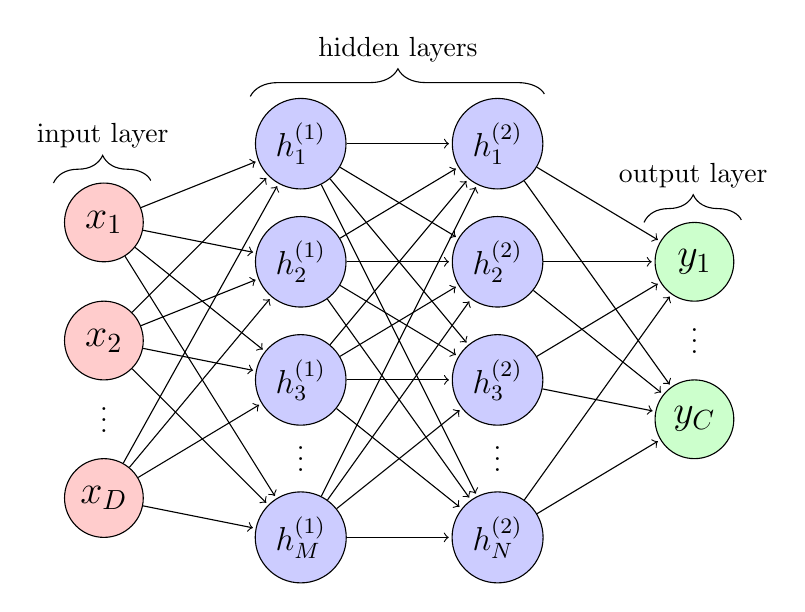
\begin{tikzpicture}[shorten >=1pt]
	\tikzstyle{unit}=[draw,shape=circle,minimum size=1.0cm]
	
	%\node[unit,fill=red!20](x1) at (0,5.0){\Large $x_1$};
	\node[unit,fill=red!20](x1) at (0,3.5){\Large $x_1$};
	\node[unit,fill=red!20](x2) at (0,2){\Large $x_2$};
	\node(dots) at (0,1.1){\vdots};
	\node[unit,fill=red!20](xd) at (0,0){\Large $x_D$};
	
	%\node[unit,fill=blue!20](w11) at (2.5,6.0){\large $h_1^{(1)}$};
	\node[unit,fill=blue!20](h11) at (2.5,4.5){\large $h_1^{(1)}$};
	\node[unit,fill=blue!20](h12) at (2.5,3.0){\large $h_2^{(1)}$};
	\node[unit,fill=blue!20](h13) at (2.5,1.5){\large $h_3^{(1)}$};
	\node(dots) at (2.5,0.6){\vdots};
	\node[unit,fill=blue!20](h1m) at (2.5,-0.5){\large $h_M^{(1)}$};
	
	%\node[unit,fill=blue!20](w21) at (5,6.0){\large $h_1^{(2)}$};
	\node[unit,fill=blue!20](h21) at (5,4.5){\large $h_1^{(2)}$};
	\node[unit,fill=blue!20](h22) at (5,3.0){\large $h_2^{(2)}$};
	\node[unit,fill=blue!20](h23) at (5,1.5){\large $h_3^{(2)}$};
	\node(dots) at (5,0.6){\vdots};
	\node[unit,fill=blue!20](h2n) at (5,-0.5){\large $h_N^{(2)}$};
	
	%\node[unit,fill=green!20](y1) at (7.5,4.5){\Large $y_1$};
	\node[unit,fill=green!20](y1) at (7.5,3.0){\Large $y_1$};
	\node(dots) at (7.5,2.1){\vdots};
	\node[unit,fill=green!20](yc) at (7.5,1.0){\Large $y_C$};
	
	% input to hidden1
	\draw[->] (x1) -- (h11);
	\draw[->] (x1) -- (h12);
	\draw[->] (x1) -- (h13);
	%\draw[->] (x1) -- (h14);
	\draw[->] (x1) -- (h1m);
	
	\draw[->] (x2) -- (h11);
	\draw[->] (x2) -- (h12);
	\draw[->] (x2) -- (h13);
	%\draw[->] (x2) -- (h14);
	\draw[->] (x2) -- (h1m);
	
	%\draw[->] (x3) -- (h11);
	%\draw[->] (x3) -- (h12);
	%\draw[->] (x3) -- (h13);
	%\draw[->] (x3) -- (h14);
	%\draw[->] (x3) -- (h1m);
	
	\draw[->] (xd) -- (h11);
	\draw[->] (xd) -- (h12);
	\draw[->] (xd) -- (h13);
	%\draw[->] (xd) -- (h14);
	\draw[->] (xd) -- (h1m);
	
	% hidden1 to hidden2
	\draw[->] (h11) -- (h21);
	\draw[->] (h11) -- (h22);
	\draw[->] (h11) -- (h23);
	%\draw[->] (h11) -- (h24);
	\draw[->] (h11) -- (h2n);
	
	\draw[->] (h12) -- (h21);
	\draw[->] (h12) -- (h22);
	\draw[->] (h12) -- (h23);
	%\draw[->] (h12) -- (h24);
	\draw[->] (h12) -- (h2n);
	
	\draw[->] (h13) -- (h21);
	\draw[->] (h13) -- (h22);
	\draw[->] (h13) -- (h23);
	%\draw[->] (h13) -- (h24);
	\draw[->] (h13) -- (h2n);
	
	%\draw[->] (h14) -- (h21);
	%\draw[->] (h14) -- (h22);
	%\draw[->] (h14) -- (h23);
	%\draw[->] (h14) -- (h24);
	%\draw[->] (h14) -- (h2n);
	
	\draw[->] (h1m) -- (h21);
	\draw[->] (h1m) -- (h22);
	\draw[->] (h1m) -- (h23);
	%\draw[->] (w1m) -- (h24);
	\draw[->] (h1m) -- (h2n);
	
	% hidden2 to output
	\draw[->] (h21) -- (y1);
	%\draw[->] (h21) -- (y2);
	\draw[->] (h21) -- (yc);
	
	\draw[->] (h22) -- (y1);
	%\draw[->] (h22) -- (y2);
	\draw[->] (h22) -- (yc);
	
	\draw[->] (h23) -- (y1);
	%\draw[->] (h23) -- (y2);
	\draw[->] (h23) -- (yc);
	
	%\draw[->] (h24) -- (y1);
	%\draw[->] (h24) -- (y2);
	%\draw[->] (h24) -- (yc);
	
	\draw[->] (h2n) -- (y1);
	%\draw[->] (h2n) -- (y2);
	\draw[->] (h2n) -- (yc);
	\draw [decorate,decoration={brace,amplitude=10pt},xshift=-4pt,yshift=0pt] (-0.5,4.0) -- (0.75,4.0) node [black,midway,yshift=+0.6cm]{input layer};
	\draw [decorate,decoration={brace,amplitude=10pt},xshift=-4pt,yshift=0pt] (2.0,5.1) -- (5.75,5.1) node [black,midway,yshift=+0.6cm]{hidden layers};
	\draw [decorate,decoration={brace,amplitude=10pt},xshift=-4pt,yshift=0pt] (7.0,3.5) -- (8.25,3.5) node [black,midway,yshift=+0.6cm]{output layer};
\end{tikzpicture}
	}
	\captionsetup{width=.9\linewidth}
	\caption{Illustration of MLP with two hidden layers.}
	\vspace{-3mm}
	\label{fig:mlp}
\end{wrapfigure}
\paragraph{Multilayer Perceptrons.} The simplest form of feedforward neural networks is the MLP based on the Perceptron~\cite{rosenblatt1958perceptron}. Basically, MLPs consist of multiple hidden layers performing matrix multiplication to extract intermediate representations of the input. Each matrix multiplication is followed by an activation function, such as the Rectified Linear Unit (ReLU) activation, which is an essential step for enabling neural networks to learn non-linear functions. Figure \ref{fig:mlp} shows an illustration of an MLP with two hidden layers. The edges between two columns of units represent the matrix multiplication where each edge corresponds to a parameter in the network. The hidden layers are often called fully-connected layers in MLPs. 

%The parameters are updated to approximate the function of interest as accurately as possible given some learning criterion which we will introduce later.  



\begin{figure}[t]
	\centering
	\resizebox{0.95\textwidth}{!}{
		

\tikzset{
	path image/.style={
		path picture={
			\node at (path picture bounding box.center) {
				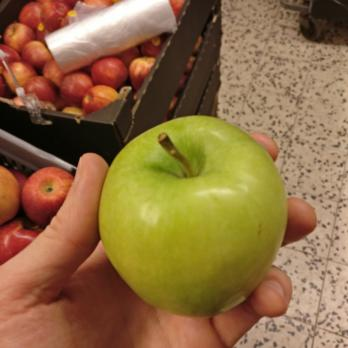
\includegraphics[height=1cm]{Chapter2/tikz/Golden-Delicious_031.jpg}};}},
}

\begin{tikzpicture}
	%\node at (0.5,-1){\begin{tabular}{c}input image\\layer $l = 0$\end{tabular}};
	\node at (0.5,2){\begin{tabular}{l}{\sf Inputs} \end{tabular}};
	\node at (2.,2){\begin{tabular}{l}{\sf Conv1} \end{tabular}};
	\node at (4.25,2){\begin{tabular}{l}{\sf Pooling1} \end{tabular}};
	\node at (6.2,2){\begin{tabular}{l}{\sf Conv2} \end{tabular}};
	\node at (8.8,2){\begin{tabular}{l}{\sf Pooling2} \end{tabular}};
	\node at (11.25,2){\begin{tabular}{l}{\sf FC} \end{tabular}};
	\node at (13.25,2){\begin{tabular}{l}{\sf Outputs} \end{tabular}};
	
	%\draw (0,0) -- (1,0) -- (1,1) -- (0,1) -- (0,0);
	\draw [path image,draw=black, thick] (0,0) rectangle (1,1);
	
	%\node at (3,3.5){\begin{tabular}{c}convolutional layer\\with non-linearities\\layer $l = 1$\end{tabular}};
	
	%\draw[fill=black,opacity=0.8,draw=black] (2.75,1.25) -- (3.75,1.25) -- (3.75,2.25) -- (2.75,2.25) -- (2.75,1.25);
	%\draw[fill=black,opacity=0.8,draw=black] (2.5,1) -- (3.5,1) -- (3.5,2) -- (2.5,2) -- (2.5,1);
	%\draw[fill=black,opacity=0.8,draw=black] (2.25,0.75) -- (3.25,0.75) -- (3.25,1.75) -- (2.25,1.75) -- (2.25,0.75);
	%\draw[fill=black,opacity=0.8,draw=black] (2,0.5) -- (3,0.5) -- (3,1.5) -- (2,1.5) -- (2,0.5);
	%\draw[fill=black,opacity=0.8,draw=black] (1.75,0.25) -- (2.75,0.25) -- (2.75,1.25) -- (1.75,1.25) -- (1.75,0.25);
	
	\draw[fill=black!50,opacity=0.8,draw=black] (2.0,0.5) -- (3.0,0.5) -- (3.0,1.5) -- (2.0,1.5) -- (2.0,0.5);
	\draw[fill=black!10,opacity=0.8,draw=black] (1.9,0.4) -- (2.9,0.4) -- (2.9,1.4) -- (1.9,1.4) -- (1.9,0.4);
	\draw[fill=black!50,opacity=0.8,draw=black] (1.8,0.3) -- (2.8,0.3) -- (2.8,1.3) -- (1.8,1.3) -- (1.8,0.3);
	\draw[fill=black!10,opacity=0.8,draw=black] (1.7,0.2) -- (2.7,0.2) -- (2.7,1.2) -- (1.7,1.2) -- (1.7,0.2);
	\draw[fill=black!50,opacity=0.8,draw=black] (1.6,0.1) -- (2.6,0.1) -- (2.6,1.1) -- (1.6,1.1) -- (1.6,0.1);
	\draw[fill=black!10,opacity=0.8,draw=black] (1.5,0) -- (2.5,0) -- (2.5,1) -- (1.5,1) -- (1.5,0);
	% conv box
	\draw (0.6,0.5) -- (0.8,0.5) -- (0.8,0.7) -- (0.6,0.7) -- (0.6,0.5);
	
	\draw (0.8,0.5) -- (2.2,0.6);
	\draw (0.8,0.7) -- (2.2,0.6);
	
	%\node at (4.5,-1){\begin{tabular}{c}subsampling layer\\layer $l = 3$\end{tabular}};
	
	%\draw[fill=black,opacity=0.8,draw=black] (5,1.25) -- (5.75,1.25) -- (5.75,2) -- (5,2) -- (5,1.25);
	%\draw[fill=black,opacity=0.8,draw=black] (4.75,1) -- (5.5,1) -- (5.5,1.75) -- (4.75,1.75) -- (4.75,1);
	%\draw[fill=black,opacity=0.8,draw=black] (4.5,0.75) -- (5.25,0.75) -- (5.25,1.5) -- (4.5,1.5) -- (4.5,0.75);
	%\draw[fill=black,opacity=0.8,draw=black] (4.25,0.5) -- (5,0.5) -- (5,1.25) -- (4.25,1.25) -- (4.25,0.5);
	%\draw[fill=black,opacity=0.8,draw=black] (4,0.25) -- (4.75,0.25) -- (4.75,1) -- (4,1) -- (4,0.25);
	%\draw[fill=black,opacity=0.8,draw=black] (3.75,0) -- (4.5,0) -- (4.5,0.75) -- (3.75,0.75) -- (3.75,0);
	
	\draw[fill=black!50,opacity=0.8,draw=black] (4.25,0.5) -- (5.0,0.5) -- (5.0,1.25) -- (4.25,1.25) -- (4.25,0.5);
	\draw[fill=black!10,opacity=0.8,draw=black] (4.15,0.4) -- (4.9,0.4) -- (4.9,1.15) -- (4.15,1.15) -- (4.15,0.4);
	\draw[fill=black!50,opacity=0.8,draw=black] (4.05,0.3) -- (4.8,0.3) -- (4.8,1.05) -- (4.05,1.05) -- (4.05,0.3);
	\draw[fill=black!10,opacity=0.8,draw=black] (3.95,0.2) -- (4.7,0.2) -- (4.7,0.95) -- (3.95,0.95) -- (3.95,0.2);
	\draw[fill=black!50,opacity=0.8,draw=black] (3.85,0.1) -- (4.6,0.1) -- (4.6,0.85) -- (3.85,0.85) -- (3.85,0.1);
	\draw[fill=black!10,opacity=0.8,draw=black] (3.75,0) -- (4.5,0) -- (4.5,0.75) -- (3.75,0.75) -- (3.75,0);
	
	% pooling box
	\draw (1.6,0.1) -- (1.8,0.1) -- (1.8,0.3) -- (1.6,0.3) -- (1.6,0.1);
	
	\draw (1.8,0.1) -- (3.9,0.15);
	\draw (1.8,0.3) -- (3.9,0.15);
	
	%\node at (7,3.5){\begin{tabular}{c}convolutional layer\\with non-linearities\\layer $l = 4$\end{tabular}};
	
	%\draw[fill=black,opacity=0.8,draw=black] (7.5,1.75) -- (8.25,1.75) -- (8.25,2.5) -- (7.5,2.5) -- (7.5,1.75);
	%\draw[fill=black,opacity=0.8,draw=black] (7.25,1.5) -- (8,1.5) -- (8,2.25) -- (7.25,2.25) -- (7.25,1.5);
	%\draw[fill=black,opacity=0.8,draw=black] (7,1.25) -- (7.75,1.25) -- (7.75,2) -- (7,2) -- (7,1.25);
	%\draw[fill=black,opacity=0.8,draw=black] (6.75,1) -- (7.5,1) -- (7.5,1.75) -- (6.75,1.75) -- (6.75,1);
	%\draw[fill=black,opacity=0.8,draw=black] (6.5,0.75) -- (7.25,0.75) -- (7.25,1.5) -- (6.5,1.5) -- (6.5,0.75);
	%\draw[fill=black,opacity=0.8,draw=black] (6.25,0.5) -- (7,0.5) -- (7,1.25) -- (6.25,1.25) -- (6.25,0.5);
	%\draw[fill=black,opacity=0.8,draw=black] (6,0.25) -- (6.75,0.25) -- (6.75,1) -- (6,1) -- (6,0.25);
	%\draw[fill=black,opacity=0.8,draw=black] (5.75,0) -- (6.5,0) -- (6.5,0.75) -- (5.75,0.75) -- (5.75,0);
	
	\draw[fill=black!50,opacity=0.8,draw=black] (6.65,0.9) -- (7.4,0.9) -- (7.4,1.65) -- (6.65,1.65) -- (6.65,0.9);			
	\draw[fill=black!10,opacity=0.8,draw=black] (6.55,0.8) -- (7.3,0.8) -- (7.3,1.55) -- (6.55,1.55) -- (6.55,0.8);			
	\draw[fill=black!50,opacity=0.8,draw=black] (6.45,0.7) -- (7.2,0.7) -- (7.2,1.45) -- (6.45,1.45) -- (6.45,0.7);	
	\draw[fill=black!10,opacity=0.8,draw=black] (6.35,0.6) -- (7.1,0.6) -- (7.1,1.35) -- (6.35,1.35) -- (6.35,0.6);		
	\draw[fill=black!50,opacity=0.8,draw=black] (6.25,0.5) -- (7.0,0.5) -- (7.0,1.25) -- (6.25,1.25) -- (6.25,0.5);
	\draw[fill=black!10,opacity=0.8,draw=black] (6.15,0.4) -- (6.9,0.4) -- (6.9,1.15) -- (6.15,1.15) -- (6.15,0.4);
	\draw[fill=black!50,opacity=0.8,draw=black] (6.05,0.3) -- (6.8,0.3) -- (6.8,1.05) -- (6.05,1.05) -- (6.05,0.3);
	\draw[fill=black!10,opacity=0.8,draw=black] (5.95,0.2) -- (6.7,0.2) -- (6.7,0.95) -- (5.95,0.95) -- (5.95,0.2);
	\draw[fill=black!50,opacity=0.8,draw=black] (5.85,0.1) -- (6.6,0.1) -- (6.6,0.85) -- (5.85,0.85) -- (5.85,0.1);
	\draw[fill=black!10,opacity=0.8,draw=black] (5.75,0) -- (6.5,0) -- (6.5,0.75) -- (5.75,0.75) -- (5.75,0);
	
	% conv box
	\draw (3.95,0.45) -- (4.15,0.45) -- (4.15,0.65) -- (3.95,0.65) -- (3.95,0.45);
	
	\draw (4.15,0.45) -- (6.05,0.55);
	\draw (4.15,0.65) -- (6.05,0.55);
	
	%\node at (9.5,-1){\begin{tabular}{c}subsampling layer\\layer $l = 6$\end{tabular}};
	
	%\draw[fill=black,opacity=0.8,draw=black] (10,1.75) -- (10.5,1.75) -- (10.5,2.25) -- (10,2.25) -- (10,1.75);
	%\draw[fill=black,opacity=0.8,draw=black] (9.75,1.5) -- (10.25,1.5) -- (10.25,2) -- (9.75,2) -- (9.75,1.5);
	%\draw[fill=black,opacity=0.8,draw=black] (9.5,1.25) -- (10,1.25) -- (10,1.75) -- (9.5,1.75) -- (9.5,1.25);
	%\draw[fill=black,opacity=0.8,draw=black] (9.25,1) -- (9.75,1) -- (9.75,1.5) -- (9.25,1.5) -- (9.25,1);
	%\draw[fill=black,opacity=0.8,draw=black] (9,0.75) -- (9.5,0.75) -- (9.5,1.25) -- (9,1.25) -- (9,0.75);
	%\draw[fill=black,opacity=0.8,draw=black] (8.75,0.5) -- (9.25,0.5) -- (9.25,1) -- (8.75,1) -- (8.75,0.5);
	%\draw[fill=black,opacity=0.8,draw=black] (8.5,0.25) -- (9,0.25) -- (9,0.75) -- (8.5,0.75) -- (8.5,0.25);
	%\draw[fill=black,opacity=0.8,draw=black] (8.25,0) -- (8.75,0) -- (8.75,0.5) -- (8.25,0.5) -- (8.25,0);
	\draw[fill=black!50,opacity=0.8,draw=black] (9.15,0.9) -- (9.65,0.9) -- (9.65,1.4) -- (9.15,1.4) -- (9.15,0.9);
	\draw[fill=black!10,opacity=0.8,draw=black] (9.05,0.8) -- (9.55,0.8) -- (9.55,1.3) -- (9.05,1.3) -- (9.05,0.8);
	\draw[fill=black!50,opacity=0.8,draw=black] (8.95,0.7) -- (9.45,0.7) -- (9.45,1.2) -- (8.95,1.2) -- (8.95,0.7);
	\draw[fill=black!10,opacity=0.8,draw=black] (8.85,0.6) -- (9.35,0.6) -- (9.35,1.1) -- (8.85,1.1) -- (8.85,0.6);
	\draw[fill=black!50,opacity=0.8,draw=black] (8.75,0.5) -- (9.25,0.5) -- (9.25,1.0) -- (8.75,1.0) -- (8.75,0.5);
	\draw[fill=black!10,opacity=0.8,draw=black] (8.65,0.4) -- (9.15,0.4) -- (9.15,0.9) -- (8.65,0.9) -- (8.65,0.4);
	\draw[fill=black!50,opacity=0.8,draw=black] (8.55,0.3) -- (9.05,0.3) -- (9.05,0.8) -- (8.55,0.8) -- (8.55,0.3);
	\draw[fill=black!10,opacity=0.8,draw=black] (8.45,0.2) -- (8.95,0.2) -- (8.95,0.7) -- (8.45,0.7) -- (8.45,0.2);
	\draw[fill=black!50,opacity=0.8,draw=black] (8.35,0.1) -- (8.85,0.1) -- (8.85,0.6) -- (8.35,0.6) -- (8.35,0.1);
	\draw[fill=black!10,opacity=0.8,draw=black] (8.25,0) -- (8.75,0) -- (8.75,0.5) -- (8.25,0.5) -- (8.25,0);
	
	% pooling box
	\draw (6.2,0.1) -- (6.4,0.1) -- (6.4,0.3) -- (6.2,0.3) -- (6.2,0.1);
	
	\draw(6.4,0.1) -- (8.65,0.15);
	\draw (6.4,0.3) -- (8.65,0.15);
	
	%\node at (12,3.5){\begin{tabular}{c}fully connected layer\\layer $l = 7$\end{tabular}};
	
	%\draw[fill=black,draw=black,opacity=0.5] (10.5,0) -- (11,0) -- (12.5,1.75) -- (12,1.75) -- (10.5,0);
	\draw[fill=black!10,draw=black,opacity=0.8] (10.5,0.1) -- (11,0.1) -- (11.8,1.0) -- (11.3,1.) -- (10.5,0.1);
	
	% flatten lines
	\draw(8.75,0.0) -- (10.5,0.1);
	\draw(9.65,1.4) -- (11.3,1.0);
	%\draw (6.4,0.3) -- (8.65,0.15);
	
	%\node at (13,-1){\begin{tabular}{c}fully connected layer\\output layer $l = 8$\end{tabular}};
	
	\draw[fill=black!10,draw=black,opacity=0.8] (12.5,0.0) -- (13,0.0) -- (13.45,0.6) -- (12.95,0.6) -- (12.5,0.0);
	
	% fc lines
	\draw(11.0,0.1) -- (12.5,0.0);
	\draw(11.8,1.0) -- (12.95,0.6);
\end{tikzpicture}
	}
	\caption{Simple CNN architecture with two convolutional layers (Conv) for extracting feature maps, two subsampling layers performing a pooling operation (Pooling), and one fully-connected layer (FC) to produce the network output. Figure inspiration from \footnotesize{\url{https://davidstutz.de/illustrating-convolutional-neural-networks-in-latex-with-tikz/}}. }
	\label{fig:cnn_simple}
\end{figure}

\vspace{-3mm}
\paragraph{Convolutional Neural Networks.} 
Convolutional layers consist of a set of filters defined by adaptable parameters to capture relationships between neighboring features in the data~\cite{lecun1998gradient}. %Convolutional layers consist of a set of filters with adaptable parameters to capture relationships between neighboring features in the data~\cite{lecun1998gradient}. 
Extracting the feature representations from one layer corresponds to convolving the input data with all filters, where the parameters in each filter are shared across every spatial location of the input. 
%Corresponding to convolving the data with a filter defined by these parameters
%The parameters in every filter are shared across every spatial location in the data when extracting the succeeding feature representation. 
This design choice enables each filter to extract important features at any position in the data. Furthermore, parameter sharing also reduces the amount of parameters in the network and lowers the number of operations for computing the outputs. Figure \ref{fig:cnn_simple} shows an illustration of a CNN architecture. Each filter slides across the width and height of the input to compute dot products between the filter weights and the local input region to produce a 2-dimensional feature map. The feature maps from all filters are then stacked depth-wise to obtain the output volume, which are often subsampled along their spatial dimensions with a pooling operation after a non-linear activation function. The feature maps in the last subsampling layer are flattened and fed into an arbitrary number of fully-connected layers (an MLP) to produce the final output. 


\vspace{-3mm}
\begin{wrapfigure}{r}{0.39\textwidth}
	\centering
	\vspace{-3mm}
	\resizebox{0.39\textwidth}{!}{
		
    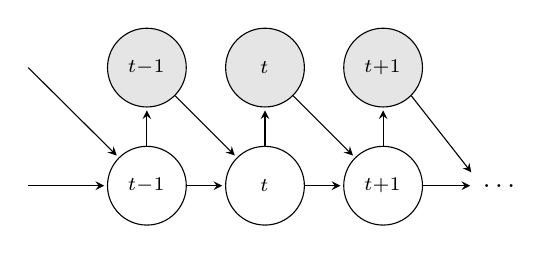
\begin{tikzpicture}[shorten >=1pt]
	\tikzstyle{unit}=[draw,shape=circle,minimum size=1.0cm]
	%\tikzstyle{box}=[draw,shape=rectangle,minimum size=1.0cm,rounded corners]
	
	\node[unit,fill=black!10](xtm1) at (0,1.5){$\vx_{t-1}$};
	\node[unit,fill=black!10](xt) at (1.5,1.5){$\vx_{t}$};
	\node[unit,fill=black!10](xtp1) at (3.0,1.5){$\vx_{t+1}$};
	
	\node[unit,fill=white](htm1) at (0,0){$\vh_{t-1}$};
	\node[unit,fill=white](ht) at (1.5,0){$\vh_{t}$};
	\node[unit,fill=white](htp1) at (3.0,0){$\vh_{t+1}$};
	
	\node (dots) at (4.5,0){\dots};
	
	\draw[-stealth] ([xshift=-1.0cm]xtm1.west) -> (htm1.north west); 
	\draw[-stealth] ([xshift=-1.0cm]htm1.west) -> (htm1.west); 
	
	\draw[-stealth] (htm1.north) -> (xtm1.south); 
	\draw[-stealth] (ht.north) -> (xt.south); 
	\draw[-stealth] (htp1.north) -> (xtp1.south); 
	
	\draw[-stealth] (htm1.east) -> (ht.west); 
	\draw[-stealth] (ht.east) -> (htp1.west); 
	\draw[-stealth] (htp1.east) -> (dots.west); 
	
	\draw[-stealth] (xtm1.south east) -> (ht.north west);
	\draw[-stealth] (xt.south east) -> (htp1.north west);
	\draw[-stealth] (xtp1.south east) -> (dots.north west);
	
\end{tikzpicture}
	}
	\captionsetup{width=.95\linewidth}
	\caption{Graphical representation of RNN.}
	\vspace{-3mm}
	\label{fig:rnn}
\end{wrapfigure}
\paragraph{Recurrent Neural Networks.} RNNs are a family of neural network models specialized for processing sequences of data. These networks predicts the next output given the past sequence and uses an extension of backpropagation to compute gradients across different time steps. 
Similar to CNNs, RNNs apply parameter sharing across time steps to enable extracting relevant information that can appear at different positions in the sequence. RNNs makes an assumption that all relevant information about the past sequence $\vx_{1:t-1}$ can be summarized in a hidden state $\vh_t$. The state evolves over time through the updated equation $\vh_t = f_{\vtheta}(\vh_{t-1}, \vx_{t-1})$ where $f_{\vtheta}$ is a neural network for capturing the long-term dependencies. Common choices for this network are the Long Short-Term Memory (LSTM)~\cite{hochreiter1997long} and Gated Recurrent Unit (GRU)~\cite{chung2014empirical} which use gating functions for determining what information is relevant for the future time steps. Figure \ref{fig:rnn} shows a graphical representation of an RNN. The initial hidden state $\vh_0$ is usually set to zero or learned. 

\vspace{3mm}
\noindent Attention-based network architectures, such as Transformers~\cite{vaswani2017attention, dosovitskiy2020image} and Graph Neural Networks~\cite{battaglia2018relational, zhou2020graph}, are not covered in this thesis; we refer the reader to the provided references for information on these networks.



\subsection{Deep Autoencoders}\label{sec:deep_autoencoders}

\begin{wrapfigure}{r}{0.42\textwidth}
	\centering
	\vspace{-3mm}
	\resizebox{0.39\textwidth}{!}{
		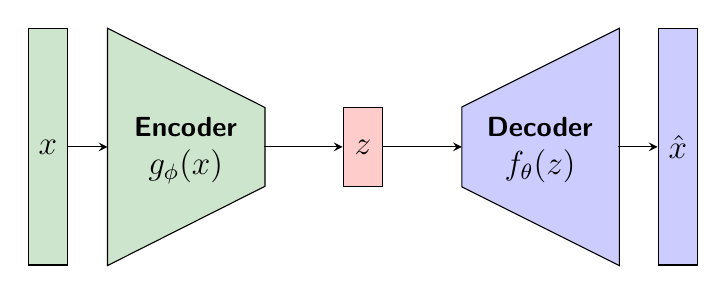
\begin{tikzpicture}
	%\node at (0.0,2.0){\begin{tabular}{c}{\sf Inputs} \end{tabular}};
	%\node at (8.0,2.0){\begin{tabular}{c}{\sf Reconstructed \\ \sf Inputs} \end{tabular}};
	
	\node[fill=Green!20, minimum width=0.5cm, minimum height=3.0cm, draw] (x) at (0,0) {\large $\boldsymbol x$};
	
	\draw[fill=Green!20] ([xshift=0.5cm]x.north east) -- ([xshift=2.5cm,yshift=0.5cm]x.east) -- ([xshift=2.5cm,yshift=-0.5cm]x.east) -- ([xshift=0.5cm]x.south east) -- cycle; 
	\node at (1.75,0.25) {{\sf \textbf{Encoder}}};
	\node at (1.75,-0.25) {\large $g_{\boldsymbol{\phi}}(\boldsymbol{x})$};
	
	\node[fill=red!20, minimum width=0.5cm, minimum height=1.0cm, draw] (z) at (4.0cm,0.0) {\large $\boldsymbol z$};
	
	\draw[fill=blue!20] ([xshift=1.0cm]z.north east) -- ([xshift=3.0cm,yshift=1.0cm]z.north east) -- ([xshift=3.0cm,yshift=-1.0cm]z.south east) -- ([xshift=1.0cm]z.south east) -- cycle;
	\node at (6.25,0.25) {{\sf \textbf{Decoder}}};
	\node at (6.25,-0.25) {\large $f_{\boldsymbol{\theta}}(\boldsymbol{z})$};
	
	\node[fill=blue!20, minimum width=0.5cm, minimum height=3.0cm, draw] (xhat) at (8.0cm,0) {\large $\boldsymbol{\hat{x}}$};
	
	\draw[-stealth] (x.east) -> ([xshift=0.5cm]x.east);
	\draw[-stealth] ([xshift=-1.0cm]z.west) -> (z.west);
	\draw[-stealth] (z.east) -> ([xshift=1.0cm]z.east);
	\draw[-stealth] ([xshift=-0.5cm]xhat.west) -> (xhat.west);
\end{tikzpicture}
	}
	\captionsetup{width=.95\linewidth}
	\caption{Illustration of an autoencoder network.}
	\label{fig:autoencoder}
	\vspace{-3mm}
\end{wrapfigure}
A common network architecture for learning latent representations of high-dimensional data in unsupervised fashions with deep learning are autoencoders. These architectures are typically built using two networks called decoder $f_{\vtheta}$ and encoder $g_{\vphi}$ with a bottleneck layer between the networks that extracts a low-dimensional representation $\vz$ of the data $\vx$. The idea is that the learned representation $\vz$ should contain enough relevant information for reconstructing the input data. Figure \ref{fig:autoencoder} shows an illustration of an autoencoder network. The encoder extracts the latent representation with $\vz = g_{\vphi}(\vx)$, while the decoder aims to reconstruct the original input, such that $\hat{\vx} = f_{\vtheta}(\vz)$ where $\hat{\vx} \approx \vx$. There exist various autoencoder approaches for improving the quality of the learned representations. For example, denoising autoencoders~\cite{vincent2008extracting} adds noise to the input data to avoid overfitting, and sparse autoencoders~\cite{ng2011sparse} induces adds sparsity constraints on the activation functions to improve robustness.



\begin{comment}

\begin{figure}[t]
	\centering
	\resizebox{0.6\textwidth}{!}{
		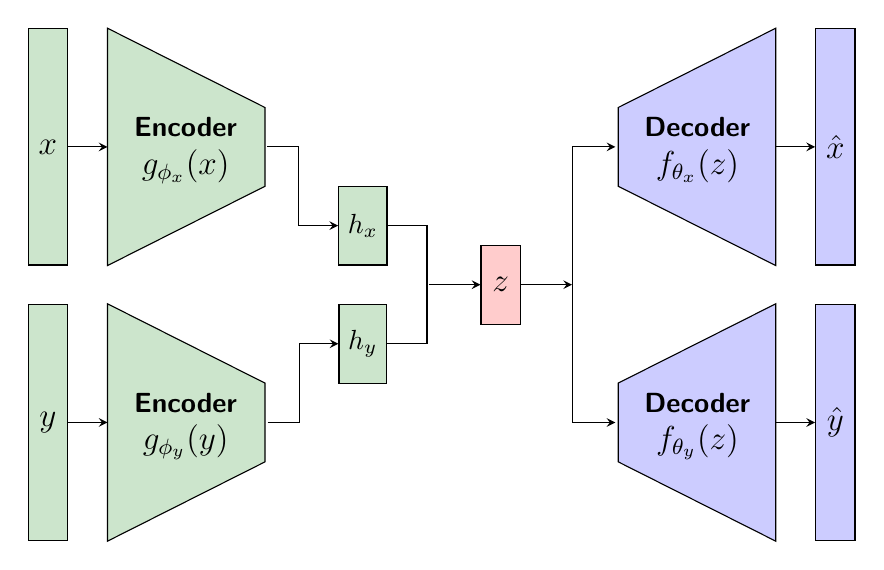
\begin{tikzpicture}
	
	\node[fill=Green!20, minimum width=0.5cm, minimum height=3.0cm, draw] (y) at (0,0) {\large $\boldsymbol y$};
	
	\node[fill=Green!20, minimum width=0.5cm, minimum height=3.0cm, draw] (x) at (0,3.5) {\large $\boldsymbol x$};
	
	\draw[fill=Green!20] ([xshift=0.5cm]x.north east) -- ([xshift=2.5cm,yshift=0.5cm]x.east) -- ([xshift=2.5cm,yshift=-0.5cm]x.east) -- ([xshift=0.5cm]x.south east) -- cycle; 
	\node at (1.75,3.75) {{\sf \textbf{Encoder}}};
	\node at (1.75,3.25) {\large $g_{\boldsymbol{\phi_x}}(\boldsymbol{x})$};
	
	
	\draw[fill=Green!20] ([xshift=0.5cm]y.north east) -- ([xshift=2.5cm,yshift=0.5cm]y.east) -- ([xshift=2.5cm,yshift=-0.5cm]y.east) -- ([xshift=0.5cm]y.south east) -- cycle; 
	\node at (1.75,0.25) {{\sf \textbf{Encoder}}};
	\node at (1.75,-0.25) {\large $g_{\boldsymbol{\phi_y}}(\boldsymbol{y})$};
	
	
	\node[fill=Green!20, minimum width=0.6cm, minimum height=1.0cm, draw] (hx) at (4.0cm,2.5cm) { $\boldsymbol{h_x}$};
	\node[fill=Green!20, minimum width=0.6cm, minimum height=1.0cm, draw] (hy) at (4.0cm,1.0cm) { $\boldsymbol{h_y}$};
	
	\node[fill=red!20, minimum width=0.5cm, minimum height=1.0cm, draw] (z) at (5.75cm,1.75cm) {\large $\boldsymbol z$};
	
	\draw[-stealth] ([xshift=-0.9cm,yshift=1.0cm]hx.west) -- ([xshift=-0.5cm,yshift=1.0cm]hx.west) |- ([xshift=-0.5cm]hx.west) -> (hx.west);
	\draw[-stealth] ([xshift=-0.9cm,yshift=-1.0cm]hy.west) -- ([xshift=-0.5cm,yshift=-1.0cm]hy.west) |- ([xshift=-0.5cm]hy.west) -> (hy.west);
	\draw (hx.east) -- ([xshift=0.5cm]hx.east) |- ([xshift=0.5cm]hy.east) -- (hy.east);
	\draw[-stealth] ([xshift=-0.65cm]z.west) -> (z.west);
	
	
	\node[fill=blue!20, minimum width=0.5cm, minimum height=3.0cm, draw] (xhat) at (10cm,3.5) {\large $\boldsymbol{\hat{x}}$};
	
	\draw[fill=blue!20] ([xshift=-0.5cm]xhat.north west) -- ([xshift=-2.5cm,yshift=0.5cm]xhat.west) -- ([xshift=-2.5cm,yshift=-0.5cm]xhat.west) -- ([xshift=-0.5cm]xhat.south west) -- cycle; 
	\node at (8.25,3.75) {{\sf \textbf{Decoder}}};
	\node at (8.25,3.25) {\large $f_{\boldsymbol{\theta_x}}(\boldsymbol{z})$};
	
	\node[fill=blue!20, minimum width=0.5cm, minimum height=3.0cm, draw] (yhat) at (10cm,0) {\large $\boldsymbol{\hat{y}}$};
	
	\draw[fill=blue!20] ([xshift=-0.5cm]yhat.north west) -- ([xshift=-2.5cm,yshift=0.5cm]yhat.west) -- ([xshift=-2.5cm,yshift=-0.5cm]yhat.west) -- ([xshift=-0.5cm]yhat.south west) -- cycle; 
	\node at (8.25,0.25) {{\sf \textbf{Decoder}}};
	\node at (8.25,-0.25) {\large $f_{\boldsymbol{\theta_y}}(\boldsymbol{z})$};
	
	\draw[-stealth] (z.east) -> ([xshift=0.65cm]z.east);
	\draw[-stealth] ([xshift=0.65cm]z.east) -- ([xshift=0.65cm,yshift=1.75cm]z.east) -> ([xshift=1.2cm,yshift=1.75cm]z.east);
	\draw[-stealth] ([xshift=0.65cm]z.east) -- ([xshift=0.65cm,yshift=-1.75cm]z.east) -> ([xshift=1.2cm,yshift=-1.75cm]z.east);
	
	\draw[-stealth] ([xshift=-0.5cm]xhat.west) -- (xhat.west);
	\draw[-stealth] ([xshift=-0.5cm]yhat.west) -- (yhat.west);
	
	\draw[-stealth] (x.east) -- ([xshift=0.5cm]x.east);
	\draw[-stealth] (y.east) -- ([xshift=0.5cm]y.east);
	
	
\end{tikzpicture}
	}
	\caption{Illustration of multimodal autoencoder network for learning joint representation $\vz$ from the different but related data types $\vx$ and $\vy$. The joint representation $\vz$ is obtained by combining the intermediate representations $\vh_{\vx}$ and $\vh_{\vy}$. %Illustration of multimodal autoencoder network for learning joint representation $\vz$ from the different but related data types $\vx$ and $\vy$. 
	}
	\label{fig:multimodal_autoencoder1}
	\vspace{-3mm}
\end{figure}
\end{comment}

\begin{wrapfigure}{r}{0.59\textwidth}
	\centering
	%\vspace{-3mm}
	\resizebox{0.54\textwidth}{!}{
		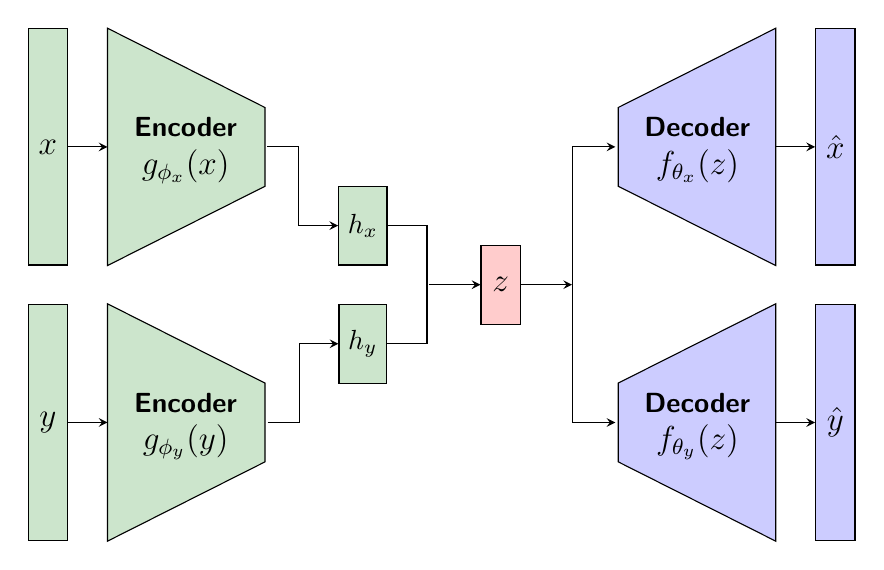
\begin{tikzpicture}
	
	\node[fill=Green!20, minimum width=0.5cm, minimum height=3.0cm, draw] (y) at (0,0) {\large $\boldsymbol y$};
	
	\node[fill=Green!20, minimum width=0.5cm, minimum height=3.0cm, draw] (x) at (0,3.5) {\large $\boldsymbol x$};
	
	\draw[fill=Green!20] ([xshift=0.5cm]x.north east) -- ([xshift=2.5cm,yshift=0.5cm]x.east) -- ([xshift=2.5cm,yshift=-0.5cm]x.east) -- ([xshift=0.5cm]x.south east) -- cycle; 
	\node at (1.75,3.75) {{\sf \textbf{Encoder}}};
	\node at (1.75,3.25) {\large $g_{\boldsymbol{\phi_x}}(\boldsymbol{x})$};
	
	
	\draw[fill=Green!20] ([xshift=0.5cm]y.north east) -- ([xshift=2.5cm,yshift=0.5cm]y.east) -- ([xshift=2.5cm,yshift=-0.5cm]y.east) -- ([xshift=0.5cm]y.south east) -- cycle; 
	\node at (1.75,0.25) {{\sf \textbf{Encoder}}};
	\node at (1.75,-0.25) {\large $g_{\boldsymbol{\phi_y}}(\boldsymbol{y})$};
	
	
	\node[fill=Green!20, minimum width=0.6cm, minimum height=1.0cm, draw] (hx) at (4.0cm,2.5cm) { $\boldsymbol{h_x}$};
	\node[fill=Green!20, minimum width=0.6cm, minimum height=1.0cm, draw] (hy) at (4.0cm,1.0cm) { $\boldsymbol{h_y}$};
	
	\node[fill=red!20, minimum width=0.5cm, minimum height=1.0cm, draw] (z) at (5.75cm,1.75cm) {\large $\boldsymbol z$};
	
	\draw[-stealth] ([xshift=-0.9cm,yshift=1.0cm]hx.west) -- ([xshift=-0.5cm,yshift=1.0cm]hx.west) |- ([xshift=-0.5cm]hx.west) -> (hx.west);
	\draw[-stealth] ([xshift=-0.9cm,yshift=-1.0cm]hy.west) -- ([xshift=-0.5cm,yshift=-1.0cm]hy.west) |- ([xshift=-0.5cm]hy.west) -> (hy.west);
	\draw (hx.east) -- ([xshift=0.5cm]hx.east) |- ([xshift=0.5cm]hy.east) -- (hy.east);
	\draw[-stealth] ([xshift=-0.65cm]z.west) -> (z.west);
	
	
	\node[fill=blue!20, minimum width=0.5cm, minimum height=3.0cm, draw] (xhat) at (10cm,3.5) {\large $\boldsymbol{\hat{x}}$};
	
	\draw[fill=blue!20] ([xshift=-0.5cm]xhat.north west) -- ([xshift=-2.5cm,yshift=0.5cm]xhat.west) -- ([xshift=-2.5cm,yshift=-0.5cm]xhat.west) -- ([xshift=-0.5cm]xhat.south west) -- cycle; 
	\node at (8.25,3.75) {{\sf \textbf{Decoder}}};
	\node at (8.25,3.25) {\large $f_{\boldsymbol{\theta_x}}(\boldsymbol{z})$};
	
	\node[fill=blue!20, minimum width=0.5cm, minimum height=3.0cm, draw] (yhat) at (10cm,0) {\large $\boldsymbol{\hat{y}}$};
	
	\draw[fill=blue!20] ([xshift=-0.5cm]yhat.north west) -- ([xshift=-2.5cm,yshift=0.5cm]yhat.west) -- ([xshift=-2.5cm,yshift=-0.5cm]yhat.west) -- ([xshift=-0.5cm]yhat.south west) -- cycle; 
	\node at (8.25,0.25) {{\sf \textbf{Decoder}}};
	\node at (8.25,-0.25) {\large $f_{\boldsymbol{\theta_y}}(\boldsymbol{z})$};
	
	\draw[-stealth] (z.east) -> ([xshift=0.65cm]z.east);
	\draw[-stealth] ([xshift=0.65cm]z.east) -- ([xshift=0.65cm,yshift=1.75cm]z.east) -> ([xshift=1.2cm,yshift=1.75cm]z.east);
	\draw[-stealth] ([xshift=0.65cm]z.east) -- ([xshift=0.65cm,yshift=-1.75cm]z.east) -> ([xshift=1.2cm,yshift=-1.75cm]z.east);
	
	\draw[-stealth] ([xshift=-0.5cm]xhat.west) -- (xhat.west);
	\draw[-stealth] ([xshift=-0.5cm]yhat.west) -- (yhat.west);
	
	\draw[-stealth] (x.east) -- ([xshift=0.5cm]x.east);
	\draw[-stealth] (y.east) -- ([xshift=0.5cm]y.east);
	
	
\end{tikzpicture}
	}
	\captionsetup{width=.95\linewidth}
	\caption{Illustration of a multimodal autoencoder network for learning a joint representation $\vz$ from the different but related data types $\vx$ and $\vy$. The joint representation $\vz$ is obtained by combining the intermediate representations $\vh_{\vx}$ and $\vh_{\vy}$.
	}
	\label{fig:multimodal_autoencoder}
	\vspace{-3mm}
\end{wrapfigure}
\paragraph{Multimodal Autoencoders.} Autoencoders can easily be extended to handling multiple types of data. The goal here is usually to learn one joint latent representation for capturing correspondences between the data types~\cite{baltruvsaitis2018multimodal}. Consider the multimodal dataset $\gD = \{(\vx_i, \vy_i)\}_{i=1}^{N}$ where $\vx$ and $\vy$ originate from two different data views (real-world images, web images) or modalities (visual signals, text descriptions) that share some high-level information. For example, $\vx$ could be an image of a living room and $\vy$ is a text sentence describing the appearance of the room, where objects are located etc. 
Figure \ref{fig:multimodal_autoencoder} shows an illustration of the network architecture. The input $\vx$ and $\vy$ have two separate encoders, $g_{\vphi_{\vx}}(\vx)$ and $g_{\vphi_{\vy}}(\vy)$, that extracts the intermediate latent representations $\vh_{\vx}$ and $\vh_{\vy}$ respectively. The intermediate representations are then combined into the joint latent representation $\vz$, often through some element-wise operation (addition, multiplication) or concatenation. The joint multimodal representation $\vz$ is then passed through two separate decoder networks, $f_{\vtheta_{\vx}}(\vz)$ and $f_{\vtheta_{\vy}}(\vz)$, for predicting the original input data separately. 
Combining different modalities, such as images, natural language, and audio signals, with autoencoders for learning more rich representations of data has been studied frequently the last decade~\cite{baltruvsaitis2018multimodal,ngiam2011multimodal,wang2015deep,vedantam2017generative,wu2018multimodal,owens2018audio}
%Combining different modalities, such as image and video, natural language, and audio signals, with autoencoders for learning more rich representations of data has been studied frequently the last decade~\cite{owens2018audio, ngiam2011multimodal, silberer2014learning, lee2020making} [Add REFs]. 
One advantage is that the network architecture can be trained in an trained end-to-end fashion to be used for both learning representations and making predictions of the used data types.
However, a major challenge is how to handle scenarios where some data types could be missing. An option here is to learn a joint representation by using a single encoder for the data type that is available at both training and test phases that is used for predicting each data type~\cite{ngiam2011multimodal}. 
%We can also  handle missing modalities for the encoders which enables cross-modal data generation between the modalities.


%Learning representations from different types of data is a highly active research field in deep learning~\cite{baltruvsaitis2018multimodal}. Combining visual data with other modalities such as natural language and audio signals for learning more rich representations of data has been studied frequently the last decade~\cite{owens2018audio, ngiam2011multimodal, silberer2014learning, lee2020making} [Add REFs]. A common framework in such applications is to use autoencoders for incorporating information from the different data types into a single joint representation. Learning from multiple sources then opens up for capturing correspondences between the data types and obtaining better representations that can be used for downstream tasks such as classification. 

%Let $\vx$ and $\vy$ originate from two different data sources but share some high-level information. For example, $\vx$ could be an image of a living room and $\vy$ is text describing the appearance of the room, where objects are located etc. Constructing a joint representation is then done by projecting both $\vx$ and $\vy$ with separate encoder networks into the same latent space. The joint multimodal representation is then passed through two separate decoder networks used for predicting the original input data individually. The advantage of multimodal autoencoders is that they can be trained end-to-end for both learning representations as well as making predictions of the used modalities. However, a major challenge is how to handle scenarios where modalities might be missing. One option is to only encode the data modality that we know will be available at both training and test phases and then establish a joint representation by decoding two both modalities~\cite{ngiam2011multimodal}.

%Multimodal autoencoders have frequently been extended to deep generative models, mainly VAEs~\cite{wang2016deep, wu2018multimodal, shi2019variational, vedantam2017generative, suzuki2016joint}. These models are capable of generating new data through sampling from the latent space in addition to learning joint representations. Furthermore, they can handle missing modalities for the encoders which enables cross-modal data generation between the modalities. In Paper B [Add REF], we employ Variational Canonical Correlation Analysis (VCCA) for learning joint representations of natural images and web-scraped information of grocery items to facilitate learning image classifiers. 




%A common architecture type for deep learning in unsupervised learning are autoencoders for learning hidden representations of unlabeled data. Autoencoders are commonly used for dimensionality reduction of high-dimensional data, where the lower-dimensional representation can be used for classification tasks, or to visualize hidden structures in the data that are hard to reveal from the original input data. The objective of the model is to reconstruct the original input data. The network architecture is built using two networks called \textit{encoder} and \textit{decoder} with a bottleneck layer between the networks for extracting the hidden representation $\vh$. The encoder and decoder architectures can be of any neural network type, such as MLPs, CNNs, or RNNs, that fits the given dataset. The encoder is used for obtaining the hidden representation of the input data, while the decoder tries to reconstruct the original input from the obtained representation. Therefore, the idea is that the learned representation should contain the relevant information for reconstructing the data. 

%Mathematically, we denote the decoder as $f_{\vtheta}$ and the encoder as $g_{\vphi}$. The encoder extracts the hidden representation $\vh = g_{\vphi}(\vx)$ from the input $\vx$, then the decoder produces a reconstruction $\hat{\vx} = f_{\vtheta}(\vh)$ from $\vh$. We train the encoder and decoder simultaneously by minimizing a reconstruction loss $\gL(f_{\vtheta}(g_{\vphi}(\vx)), \vx)$, for instance mean-squared error loss, using SGD similarly as for the feedforward networks described above. There exist various kinds of methods for improving the quality of the learned representations in autoencoders. For example, we can adjust target task by adding noise to the inputs and let the decoder reconstruct the original input from noise variants~\cite{vincent2008extracting}, or we can induce different constraints in the bottleneck layer to, for example, obtain a sparse lower-dimensional representation of the data. Next, we will introduce the variational autoencoder which originates from latent variable models. 

\subsubsection{Variational Autoencoders}\label{sec:variational_autoencoders}

In this section, we give an overview of the variational autoencoder (VAE)~\cite{kingma2013auto, kingma2019introduction} that we apply for representation learning in Paper \ref{paperA} and \ref{paperB}. 
The VAE is a deep generative model that enable learning of data representations %learns representations of data 
by combining ideas from deep learning and probabilistic graphical models~\cite{koller2009probabilistic}. 
As commonly done in unsupervised learning, VAEs aim to learn a parametric distribution $p_{\vtheta}(\vx)$ that approximates the data distribution $p_{data}$ given a dataset $\gD = \{\vx^{(i)}\}_{i=1}^{N}$ where $\vx^{(i)} \sim p_{data}$. We frame the problem of learning $p_{\vtheta}(\vx)$ by expressing the distribution using latent variables $\vz$, such that
\begin{equation}\label{eq:px}
	p_{\vtheta}(\vx) = \int p_{\vtheta}(\vx, \vz) \, d\vz = \int p_{\vtheta}(\vx | \vz) p(\vz) \, d\vz,
\end{equation}
where the joint distribution $p_{\vtheta}(\vx, \vz)$ is the model which factorizes into the likelihood $p_{\vtheta}(\vx | \vz)$ and the prior distribution $p(\vz)$ for the latent variables. The latent variables $\vz$ are introduced for representing underlying structures and relationships in $\vx$ that can be difficult to observe from the data itself. We can view $\vz$ as containing meaningful information for the data generation process by assuming that the data was generated with the following steps: 
\begin{enumerate}[topsep=1pt,noitemsep]
	\item sample the latent vector $\vz \sim p(\vz)$ from the prior.
	\item generate data point $\vx \sim p_{\vtheta}(\vx | \vz)$ given the sampled $\vz$.
\end{enumerate}

\vspace{-3mm}
\paragraph{The Evidence Lower Bound.} The problem with learning the parameters $\vtheta$ that maximize $p_{\vtheta}(\vx)$ is that the integral in Equation \ref{eq:px} is almost always intractable due to the 
prohibitively large number of values for $\vz$ that need to be evaluated. %immense amount of values for $\vz$ that needs to be evaluated. 
Instead, we can reformulate the problem using Bayes' rule %compute $p_{\vtheta}(\vx)$ using Bayes' rule 
\begin{equation}
	p_{\vtheta}(\vx) = \frac{p_{\vtheta}(\vx | \vz) p(\vz) }{p_{\vtheta}(\vz | \vx)},
\end{equation}
where $p_{\vtheta}(\vz | \vx)$ is the posterior of $\vz$ given $\vx$ and $p_{\vtheta}(\vx | \vz)$ is the likelihood of $\vx$ given $\vz$. The posterior needs to be approximated using variational inference~\cite{zhang2018advances,blei2017variational}, where we define an approximate posterior distribution $q_{\vphi}(\vz | \vx)$ parameterized by $\vphi$ to infer the latents $\vz$.  
%where the posterior distribution $p_{\vtheta}(\vz | \vx)$ can facilitate faster learning by inferring the latents $\vz$ from data $\vx$. However, we need to resort to approximating the posterior using variational inference~\cite{zhang2018advances,blei2017variational} since the posterior needs access to $p_{\vtheta}(\vx)$ to be computed. We then define an approximate posterior distribution $q_{\vphi}(\vz | \vx)$ parameterized by $\vphi$ to infer the latents $\vz$. 
This allows us to form a lower bound on the marginal log-likelihood $\log p_{\vtheta}(\vx)$ given by 
\begin{align}\label{eq:elbo}
	\log p_{\vtheta}(\vx) \geq \E_{z \sim q_{\vphi}(\vz | \vx)}[\log p_{\vtheta}(\vx | \vz)] - \KL[q_{\vphi}(\vz |  \vx) \, || \, p(\vz)] ,
\end{align}
which is called the evidence lower bound (ELBO). The expected value over $\log p_{\vtheta}(\vx | \vz)$ can be estimated with Monte Carlo sampling using $q_{\vphi}(\vz | \vx)$, and the Kullback-Leibler (KL) divergence between $q_{\vphi}(\vz |  \vx)$ and $p(\vz)$ can be computed analytically depending on how we choose these distributions. Commonly, the approximate posterior is selected to be a Gaussian distribution $q_{\vphi}(\vz | \vx) = \gN(\vz; \vmu_{\vphi}(\vx), \text{diag}(\vsigma_{\vphi}(\vx)))$ where the parameters $\vphi$ are used for computing the mean $\vmu_{\vphi}(\vx)$ and standard deviation $\vsigma_{\vphi}(\vx)$ of the approximate posterior given $\vx$, and $\text{diag}(\cdot)$ is for constraining the covariance matrix to be a diagonal matrix. The prior distribution is also selected to be a zero-mean, standard Gaussian distribution $p(\vz) = \gN(\vz; \mathbf{0}, \mathbf{I})$ where $\mathbf{I}$ is the identity matrix. 

\begin{comment}
\begin{figure}[t]
	\centering
	\resizebox{0.6\textwidth}{!}{
		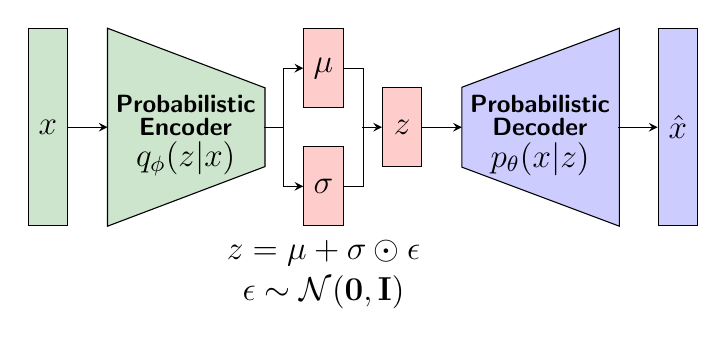
\begin{tikzpicture}
	
	
	\node[fill=Green!20, minimum width=0.5cm, minimum height=2.5cm, draw] (x) at (0,0) {\large $\boldsymbol x$};
	
	\draw[fill=Green!20] ([xshift=0.5cm]x.north east) -- ([xshift=2.5cm,yshift=0.5cm]x.east) -- ([xshift=2.5cm,yshift=-0.5cm]x.east) -- ([xshift=0.5cm]x.south east) -- cycle; 
	\node at (1.75,0.3) {{\small\sf \textbf{Probabilistic}}};
	\node at (1.75,0.0) {{\small\sf \textbf{Encoder}}};
	\node at (1.75,-0.4) {\large $q_{\boldsymbol{\phi}}(\boldsymbol{z} | \boldsymbol{x})$};
	
	\draw[-stealth] (x.east) -- ([xshift=0.5cm]x.east);
	
	\node[fill=red!20, minimum width=0.5cm, minimum height=1.0cm, draw] (mu) at (3.5cm,0.75cm) {\large $\boldsymbol{\mu}$};
	\node[fill=red!20, minimum width=0.5cm, minimum height=1.0cm, draw] (sigma) at (3.5cm,-0.75cm) {\large $\boldsymbol{\sigma}$};
	
	\node at (3.5cm,-1.6cm) {\large $\boldsymbol{z} = \boldsymbol{\mu} + \boldsymbol{\sigma} \odot \boldsymbol{\epsilon}$};
	\node at (3.5cm,-2.1cm) {\large $\boldsymbol{\epsilon} \sim \mathcal{N}(\mathbf{0}, \mathbf{I})$};
	\draw ([xshift=-0.5cm,yshift=-0.75cm]mu.west) -- ([xshift=-0.25cm,yshift=-0.75cm]mu.west);
	\draw[-stealth] ([xshift=-0.25cm,yshift=-0.75cm]mu.west) |- ([xshift=-0.25cm]mu.west) -- (mu.west);
	\draw[-stealth] ([xshift=-0.25cm,yshift=0.75cm]sigma.west) |- ([xshift=-0.25cm]sigma.west) -- (sigma.west);
	
	%\node[fill=red!20, minimum width=0.5cm, minimum height=1.0cm, draw] (z) at (5.0cm,0.0) {\large $\boldsymbol z$};
	\node[fill=red!20, minimum width=0.5cm, minimum height=1.0cm, draw] (z) at (4.5cm,0.0) {\large $\boldsymbol z$};
	\draw (mu.east) -- ([xshift=0.25cm]mu.east) |- ([xshift=-0.25cm]z.west);
	\draw (sigma.east) -- ([xshift=0.25cm]sigma.east) |- ([xshift=-0.25cm]z.west);
	\draw[-stealth] ([xshift=-0.25cm]z.west) -- (z.west);
	
	%\draw[-stealth] ([xshift=-2.5cm]z.west) -> ([xshift=-2.0cm]z.west);
	%\draw[-stealth] ([xshift=-0.5cm,yshift=-0.75cm]mu.west) -- ([xshift=-0.5cm]mu.west) |- (mu.west);
	%%%\draw[-stealth] ([xshift=-0.5cm,yshift=0.75cm]sigma.west) -- ([xshift=-0.5cm]sigma.west) |- (sigma.west);
	%%%\draw[-stealth] (mu.west) -- ([xshift=-0.5cm]mu.west) |- ([xshift=-0.5cm]sigma.west) -- (sigma.west);
	%\draw (mu.east) -- ([xshift=0.5cm]mu.east) |- ([xshift=0.5cm]sigma.east) -- (sigma.east);
	%\draw[-stealth] ([xshift=-0.45cm]z.west) -> (z.west);
	
	\draw[fill=blue!20] ([xshift=0.5cm]z.north east) -- ([xshift=2.5cm,yshift=0.75cm]z.north east) -- ([xshift=2.5cm,yshift=-0.75cm]z.south east) -- ([xshift=0.5cm]z.south east) -- cycle;
	\node at (6.25,0.3) {{\small\sf \textbf{Probabilistic}}};
	\node at (6.25,0.0) {{\small\sf \textbf{Decoder}}};
	\node at (6.25,-0.4) {\large $p_{\boldsymbol{\theta}}(\boldsymbol{x} | \boldsymbol{z})$};
	
	\node[fill=blue!20, minimum width=0.5cm, minimum height=2.5cm, draw] (xhat) at (8.0cm,0) {\large $\boldsymbol{\hat{x}}$};
	
	\draw[-stealth] (z.east) -- ([xshift=0.5cm]z.east);
	\draw[-stealth] ([xshift=-0.5cm]xhat.west) -- (xhat.west);
	
	
\end{tikzpicture}
	}
	\caption{Illustration of a VAE. 
	}
	\label{fig:vae1}
	\vspace{-3mm}
\end{figure}	
\end{comment}


\vspace{-3mm}
\begin{wrapfigure}{r}{0.48\textwidth}
	\centering
	\vspace{-2mm}
	\resizebox{0.45\textwidth}{!}{
		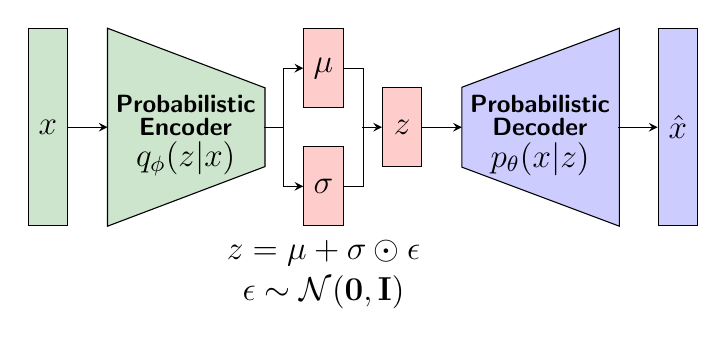
\begin{tikzpicture}
	
	
	\node[fill=Green!20, minimum width=0.5cm, minimum height=2.5cm, draw] (x) at (0,0) {\large $\boldsymbol x$};
	
	\draw[fill=Green!20] ([xshift=0.5cm]x.north east) -- ([xshift=2.5cm,yshift=0.5cm]x.east) -- ([xshift=2.5cm,yshift=-0.5cm]x.east) -- ([xshift=0.5cm]x.south east) -- cycle; 
	\node at (1.75,0.3) {{\small\sf \textbf{Probabilistic}}};
	\node at (1.75,0.0) {{\small\sf \textbf{Encoder}}};
	\node at (1.75,-0.4) {\large $q_{\boldsymbol{\phi}}(\boldsymbol{z} | \boldsymbol{x})$};
	
	\draw[-stealth] (x.east) -- ([xshift=0.5cm]x.east);
	
	\node[fill=red!20, minimum width=0.5cm, minimum height=1.0cm, draw] (mu) at (3.5cm,0.75cm) {\large $\boldsymbol{\mu}$};
	\node[fill=red!20, minimum width=0.5cm, minimum height=1.0cm, draw] (sigma) at (3.5cm,-0.75cm) {\large $\boldsymbol{\sigma}$};
	
	\node at (3.5cm,-1.6cm) {\large $\boldsymbol{z} = \boldsymbol{\mu} + \boldsymbol{\sigma} \odot \boldsymbol{\epsilon}$};
	\node at (3.5cm,-2.1cm) {\large $\boldsymbol{\epsilon} \sim \mathcal{N}(\mathbf{0}, \mathbf{I})$};
	\draw ([xshift=-0.5cm,yshift=-0.75cm]mu.west) -- ([xshift=-0.25cm,yshift=-0.75cm]mu.west);
	\draw[-stealth] ([xshift=-0.25cm,yshift=-0.75cm]mu.west) |- ([xshift=-0.25cm]mu.west) -- (mu.west);
	\draw[-stealth] ([xshift=-0.25cm,yshift=0.75cm]sigma.west) |- ([xshift=-0.25cm]sigma.west) -- (sigma.west);
	
	%\node[fill=red!20, minimum width=0.5cm, minimum height=1.0cm, draw] (z) at (5.0cm,0.0) {\large $\boldsymbol z$};
	\node[fill=red!20, minimum width=0.5cm, minimum height=1.0cm, draw] (z) at (4.5cm,0.0) {\large $\boldsymbol z$};
	\draw (mu.east) -- ([xshift=0.25cm]mu.east) |- ([xshift=-0.25cm]z.west);
	\draw (sigma.east) -- ([xshift=0.25cm]sigma.east) |- ([xshift=-0.25cm]z.west);
	\draw[-stealth] ([xshift=-0.25cm]z.west) -- (z.west);
	
	%\draw[-stealth] ([xshift=-2.5cm]z.west) -> ([xshift=-2.0cm]z.west);
	%\draw[-stealth] ([xshift=-0.5cm,yshift=-0.75cm]mu.west) -- ([xshift=-0.5cm]mu.west) |- (mu.west);
	%%%\draw[-stealth] ([xshift=-0.5cm,yshift=0.75cm]sigma.west) -- ([xshift=-0.5cm]sigma.west) |- (sigma.west);
	%%%\draw[-stealth] (mu.west) -- ([xshift=-0.5cm]mu.west) |- ([xshift=-0.5cm]sigma.west) -- (sigma.west);
	%\draw (mu.east) -- ([xshift=0.5cm]mu.east) |- ([xshift=0.5cm]sigma.east) -- (sigma.east);
	%\draw[-stealth] ([xshift=-0.45cm]z.west) -> (z.west);
	
	\draw[fill=blue!20] ([xshift=0.5cm]z.north east) -- ([xshift=2.5cm,yshift=0.75cm]z.north east) -- ([xshift=2.5cm,yshift=-0.75cm]z.south east) -- ([xshift=0.5cm]z.south east) -- cycle;
	\node at (6.25,0.3) {{\small\sf \textbf{Probabilistic}}};
	\node at (6.25,0.0) {{\small\sf \textbf{Decoder}}};
	\node at (6.25,-0.4) {\large $p_{\boldsymbol{\theta}}(\boldsymbol{x} | \boldsymbol{z})$};
	
	\node[fill=blue!20, minimum width=0.5cm, minimum height=2.5cm, draw] (xhat) at (8.0cm,0) {\large $\boldsymbol{\hat{x}}$};
	
	\draw[-stealth] (z.east) -- ([xshift=0.5cm]z.east);
	\draw[-stealth] ([xshift=-0.5cm]xhat.west) -- (xhat.west);
	
	
\end{tikzpicture}
	}
	\vspace{-2mm}
	\captionsetup{width=.95\linewidth}
	\caption{Illustration of a variational autoencoder with the reparameterization trick equation.  
	}
	\label{fig:vae}
	\vspace{-3mm}
\end{wrapfigure}
\paragraph{Network Architecture.} The VAE architecture resembles a standard autoencoder where the encoder and decoder networks are probabilistic in the sense that they output parameters of probability distributions. In contrast to autoencoders that learn latent representations $\vz$ that minimizes the reconstruction error on the data, VAEs learns an approximate posterior $q_{\vphi}(\vz | \vx)$ that maximizes the likelihood of $p_{\vtheta}(\vx)$. Similar to autoencoders, we can extract latent representations of the data with the probabilistic encoder. However, VAEs can also estimate the likelihood of unseen data points under the learned model, as well as generate new data by decoding latents sampled from the prior. 
Figure \ref{fig:vae} shows an illustration of a VAE architecture. The encoder represents the approximate posterior $q_{\vphi}(\vz | \vx)$ which outputs the mean $\vmu_{\vphi}(\vx)$ and standard deviation $\vsigma_{\vphi}(\vx)$ of a Gaussian distribution over $\vz$, which is the standard choice for $q_{\vphi}$~\cite{kingma2013auto}. The latent vector is sampled using the "reparametrization trick"~\cite{rezende2014stochastic, kingma2013auto} by computing 
\begin{equation}
	\vz = \vmu_{\vphi}(\vx) + \vsigma_{\vphi}(\vx) \odot \vepsilon, \quad \text{where} \quad \vepsilon \sim \gN(\bm{0}, \mathbf{I}),
\end{equation}
where $\odot$ denotes element-wise multiplication. The reparametrization enables computing gradients of the expectation $\E_{z \sim q_{\vphi}(\vz | \vx)}[\log p_{\vtheta}(\vx | \vz)]$ in Equation \ref{eq:elbo} with the backpropagation algorithm. The decoder represents the likelihood $p_{\vtheta}(\vx | \vz)$ that can be used to generate data $\vx$ from sampled latents $\vz$, where the distributional form depends on the data type of $\vx$. 

\vspace{3mm}
VAEs have been used in various applications for modeling images, text, and audio data~\cite{gregor2015draw, mansimov2015generating, pu2016variational, razavi2019generating, chung2015recurrent, serban2017hierarchical, li2018disentangled}.
 Furthermore, they have been extended to modeling data from different modalities due to their capability of handling missing modalities to enable cross-modal data generation~\cite{wang2016deep, wu2018multimodal, shi2019variational, vedantam2017generative, suzuki2016joint}. In Paper \ref{paperA} and \ref{paperB}, we employ Variational Canonical Correlation Analysis (VCCA)~\cite{wang2016deep} for learning joint representations of natural images and web-scraped information of grocery items to facilitate learning image classifiers. 



\begin{comment}
The variational autoencoder~\cite{kingma2013auto} (VAE) is a variant of autoencoders where learning is viewed from the perspective of probabilistic modeling. These models come from the family of deep generative models, where the goal is to approximate some underlying data distribution $p_{data}$ with a parametric distribution $p_{\vtheta}$ learned from a dataset $\gD \sim p_{data}$. A common approach for estimating $p_{\vtheta}$ is to use a latent variable model that infers hidden structures in the data to facilitate learning the distribution. VAEs is a deep latent variable model that uses neural networks for learning $p_{\vtheta}$ making the training scalable to large high-dimensional datasets. 

The main idea with introducing latent variables is that they should encode some semantically meaningful information about the observed data. Latent variable models are usually expressed by the joint distribution 
\begin{align}
	p_{\vtheta}(\vx, \vz) = p_{\vtheta}(\vx | \vz) p(\vz),
\end{align}
where $\vz$ denotes the latent variables and $\vx$ the observed variables that represents the observed data points. The distribution $p_{\vtheta}(\vx | \vz)$ is the likelihood of the data and $p(\vz)$ is the prior distribution for the latents. This model describes the generative process of the data $\vx$ by following the steps 1) sample the latent vector $\vz \sim p(\vz)$ from the prior, and 2) generate data point $\vx \sim p(\vx | \vz)$ from the sampled latent $\vz$. We are now interested in learning the model $p_{\vtheta}(\vx, \vz)$ that best fits a given dataset $\gD$, as well as inferring the posterior distribution $p_{\vtheta}(\vz | \vx)$ over the latent variables $\vz$ given the data $\vx$.

The overall goal with latent variable models is to maximize the marginal log-likelihood $\log p_{\vtheta}(\vx)$ given a dataset $\gD \sim p_{data}$. However, computing $p_{\vtheta}(\vx)$ by with marginalizing out the $\vz$ from the model $p_{\vtheta}(\vx) = \int p_{\vtheta}(\vx, \vz) \, d\vz$ is in general intractable due to the many settings of $\vz$ we would need to evaluate. Consequently, the posterior distribution also becomes intractable since $p_{\vtheta}(\vz | \vx) = p_{\vtheta}(\vx, \vz) / p_{\vtheta}(\vx)$ from Bayes' rule. Variational inference~\cite{zhang2018advances, blei2017variational} is a technique for enabling learning of latent variable models. The idea of variational inference is to provide means for calculating the marginal log-likelihood $\log p_{\vtheta}(\vx)$ by selecting a parameterized distribution $q_{\vphi}$ for approximating the true posterior distribution. In VAEs, the approximate posterior $q_{\vphi}(\vz | \vx)$ is represented as a neural network with parameters $\vphi$ that outputs the latents $\vz$ given data points $\vx$. With this approach, we can now form a lower bound on the marginal log-likelihood given by 
\begin{align}
	\log p_{\vtheta}(\vx) \geq \E_{z \sim q_{\vphi}(\vz | \vx)}[\log p_{\vtheta}(\vx | \vz)] - \KL[q_{\vphi}(\vz |  \vx) \, || \, p(\vz)] . 
\end{align}
The right-hand side is called the evidence lower bound (ELBO) and comprises of two quantities that we can evaluate to train the model. The expectation over the log-likelihood $\log p_{\vtheta}(\vx | \vz)$ can be estimated with Monte Carlo sampling. The KL divergence between $q_{\vphi}(\vz |  \vx)$ and $p(\vz)$ can be computed analytically depending on how we choose these distributions. The standard choice for the prior is to use a zero-mean unit-variance Gaussian distribution $p(\vz) = \gN(\vz; \bm{0}, \mathbf{I})$ where $\mathbf{I}$ is the identity matrix. The approximate posterior is also selected to be a Gaussian distribution $q_{\vphi}(\vz | \vx) = \gN(\vz; \vmu_{\vphi}(\vx), \text{diag}(\vsigma_{\vphi}(\vx)))$, where the encoder network parameterized by $\vphi$ outputs the the means $\vmu_{\vphi}(\vx)$ and standard deviations $\vsigma_{\vphi}(\vx)$ for the latent dimensions. The latent vector is sampled using the "reparametrization trick"~\cite{rezende2014stochastic, kingma2013auto} by computing $\vz = \vmu_{\vphi}(\vx) + \vepsilon \odot \vsigma_{\vphi}(\vx)$, where $\vepsilon \sim \gN(\bm{0}, \mathbf{I})$ and $\odot$ denotes element-wise multiplication, which enables backpropagating gradients through the sampling operation. The likelihood $p_{\vtheta}(\vx | \vz)$ is the decoder network that tries to reconstruct the original input to the encoder. The likelihood distribution depends on the type of data $\vx$ we wish to generate. If $\vx$ is a continuous variable, then we can let the decoder output Gaussian parameters for the likelihood similar as for the encoder. 

VAEs have been used in various applications for modeling images, text, and audio data, as well as when combining data from different modalities. Next, we will briefly introduce how autoencoders can be used when learning representations from multiple data types from different modalities. 

Multimodal autoencoders have frequently been extended to deep generative models, mainly VAEs~\cite{wang2016deep, wu2018multimodal, shi2019variational, vedantam2017generative, suzuki2016joint}. These models are capable of generating new data through sampling from the latent space in addition to learning joint representations. Furthermore, they can handle missing modalities for the encoders which enables cross-modal data generation between the modalities. In Paper B [Add REF], we employ Variational Canonical Correlation Analysis (VCCA) for learning joint representations of natural images and web-scraped information of grocery items to facilitate learning image classifiers. 
\end{comment}


\begin{comment}


\subsubsection{Multimodal Learning using Autoencoders}

Learning representations from different types of data is a highly active research field in deep learning~\cite{baltruvsaitis2018multimodal}. Combining visual data with other modalities such as natural language and audio signals for learning more rich representations of data has been studied frequently the last decade~\cite{owens2018audio, ngiam2011multimodal, silberer2014learning, lee2020making} [Add REFs]. A common framework in such applications is to use autoencoders for incorporating information from the different data types into a single joint representation. Learning from multiple sources then opens up for capturing correspondences between the data types and obtaining better representations that can be used for downstream tasks such as classification. 

Let $\vx$ and $\vy$ originate from two different data sources but share some high-level information. For example, $\vx$ could be an image of a living room and $\vy$ is text describing the appearance of the room, where objects are located etc. Constructing a joint representation is then done by projecting both $\vx$ and $\vy$ with separate encoder networks into the same latent space. The joint multimodal representation is then passed through two separate decoder networks used for predicting the original input data individually. The advantage of multimodal autoencoders is that they can be trained end-to-end for both learning representations as well as making predictions of the used modalities. However, a major challenge is how to handle scenarios where modalities might be missing. One option is to only encode the data modality that we know will be available at both training and test phases and then establish a joint representation by decoding two both modalities~\cite{ngiam2011multimodal}.

Multimodal autoencoders have frequently been extended to deep generative models, mainly VAEs~\cite{wang2016deep, wu2018multimodal, shi2019variational, vedantam2017generative, suzuki2016joint}. These models are capable of generating new data through sampling from the latent space in addition to learning joint representations. Furthermore, they can handle missing modalities for the encoders which enables cross-modal data generation between the modalities. In Paper B [Add REF], we employ Variational Canonical Correlation Analysis (VCCA) for learning joint representations of natural images and web-scraped information of grocery items to facilitate learning image classifiers. 

\end{comment}

%% talk about notation, then go into DQN, actor-critic methods and PPO briefly
\subsection{Deep Reinforcement Learning}\label{sec:deep_rl}


In this section, we give a brief overview RL to provide some preliminaries for Paper \ref{paperD}. The RL setup considers a learning agent that interacts with an environment $E$ over a number of discrete time steps~\cite{sutton2018reinforcement}. The environment is modeled with a Markov Decision Process (MDP)~\cite{bellman1957markovian} represented as a tuple $E = (\gS, \gA, P, R, \mu, \gamma)$ consisting of the state space $\gS$, action space $\gA$, state transition probability $P(s' | s, a)$, reward function $R(s, a)$, initial state distribution $\mu(s_1)$, and discount factor $\gamma$. At each time step $t$, the agent receives a state $s_t$ from the environment, selects an action $a_t \in \gA$ using a policy $\pi(a | s)$, and enters the next state $s_{t+1}$ with transition probability $P(s_{t+1} | s_t, a_t)$ and receives a numerical reward following $r_t$ from the environment. This procedure is repeated until the agent reaches a terminal state in which the procedure can be restarted. The return $G_t = \sum_{k=0}^{\infty} \gamma^{k} r_{t+k}$ is the discounted accumulated reward from time step $t$. The goal for the agent is to learns policy that maximizes the expected return. 

The value function $V^{\pi}(s) = \E[G_t | s_t=s]$ defines the expected return following policy $\pi$ from state $s$. Value functions are essential for learning as they can be used for comparing policies, such that $\pi \geq \pi'$ if and only if $V^{\pi}(s) \geq V^{\pi'}(s)$~\cite{sutton2018reinforcement}. An optimal policy $\pi^{*}$ is defined as a policy that is better than or equal to all other policies. There may exist several optimal policies $\pi^{*}$ that share the same optimal value function given by $V^{*}(s) = \max_{\pi} V^{\pi}(s)$ for all states $s \in \gS$. 
Similar to the value function, we also have the action value function $Q^{\pi}(s, a) = \E[G_t | s_t=s, a_t=a]$ which is the expected return for selecting action $a$ in state $s$ and following policy $\pi$. Optimal policies also share the same action value function given by $Q^{*}(s, a) = \max_{\pi} Q^{\pi}(s, a)$ for all states $s \in \gS$ and actions $a \in \gA$. The optimal action value function $Q^{*}$ can be written in terms of the optimal value function $V^{*}$ as
\begin{align}
	Q^{*}(s, a) = \E[r_{t+1} + \gamma V^{*}(s) | s_t=s, a_t=a]. 
\end{align}
This means that if we have access to $Q^{*}$, we can directly obtain the optimal action $a^*$ in state $s$ by using $a^{*} = \argmax_{a} Q^{*}(s, a)$ to maximize the expected return. 

In this thesis, we focus on model-free RL algorithms which have been popular in past years. The alternative is model-based RL algorithms which allows the agent to plan ahead when interacting with the environment by having access to a function that predicts the next states and rewards. However, having access to the ground truth of such function is impossible in many RL problems. Model-free RL algorithms can be divided into Q-learning and policy optimization methods. Q-learning methods, such as Deep Q-Networks (DQNs)~\cite{mnih2013playing, mnih2015human}, aims to approximate the optimal action value function $Q^{*}(s, a)$ with parametric function $Q_{\vtheta}(s, a)$ by minimizing objective functions based on the Bellman equation. The optimization is often performed off-policy, such that the agent can be updated using data collected from the environment at any point in time. The actions are selected with $a_t = \argmax_{a} Q^{*}(s, a)$ through the connection between the action value function and the policy.  
Policy optimization methods, such as Advantage Actor-Critic (A2C)~\cite{mnih2016asynchronous},  represent the policy in a parametric form $\pi_{\vtheta}(a | s)$. The optimization is often performed on-policy meaning that the policy is only updated using data collected in the environment by the most recent policy. Policy optimization methods tends to be more stable than Q-learning methods. However, as Q-learning methods can reuse collected data for updating the policy, these methods tends to be more sample efficient than policy optimization methods.



\begin{comment}
\vspace{-3mm}
\paragraph{Deep Q-Networks.} The Deep Q-Network (DQN)~\cite{mnih2013playing, mnih2015human} is a value-based RL algorithm which aims to approximate the optimal action value function as $Q^{*}(s, a) \approx Q_{\vtheta}(s, a)$ with a neural network $Q_{\vtheta}$ parameterized by $\vtheta$. For learning the function $Q_{\vtheta}$, we collect data from the environment with by using an epsilon-greedy policy, i.e., $a_t = \argmax_a Q_{\vtheta}(s_t, a)$, in state $s_t$. For estimating $Q_{\vtheta}$, we minimize the following loss based on the Bellman equation:
\begin{align}
	\gL_{\text{DQN}}(\vtheta) = (r_t + \gamma \max_{a'} Q_{\vtheta^{-}}(s_{t+1}, a') - Q_{\vtheta}(s_t, a_t))^2 , 
\end{align}
where $\vtheta^{-}$ is a previous copy of the network $\vtheta$ referred to as the target network. In addition to the introduction of target networks, several methods have been proposed for stabilizing the learning process, such as using experience replay~\cite{lin1992self} to sample training data stored in a replay buffer, applying L1-smoothing to the loss, correcting the action value estimates~\cite{van2016deep}, and improving generalization across actions~\cite{wang2016dueling}. 

\vspace{-3mm}
\paragraph{Policy Gradient Methods.} An alternative to value-based RL is using policy gradient methods for learning the policy. Here, the optimal policy is estimated directly with a parameterized form $\pi_{\vtheta}(a | s)$ where $\vtheta$ represents the parameters of a neural network. The policy network takes the state $s_t$ as input and outputs a distribution over the possible actions $a_t$. Policy gradient methods often use an actor-critic approach~\cite{sutton2018reinforcement,konda1999actor}, where the policy is known as the actor that selects actions, and the critic evaluates the actions made by the actor by estimating the value function $V_{\vlambda}(s_{t})$ parameterized by ${\vlambda}$. 
For updating the policy, the agent collects experiences from the environment with the current policy and aims to minimize the loss 
\begin{align}
	\gL_{\text{PG}}(\vtheta) = \E_{s_t \sim E, a_t \sim \pi_{\vtheta}}[\log \pi_{\vtheta}(a_t | s_t) \hat{A}(s_t, a_t)],
\end{align}
where $\hat{A}(s, a)$ is an estimate of the advantage function, which describes how much better or worse a taken action is on average, and is given by 
\begin{align}
	\hat{A}(s_t, a_t) = \sum_{i=0}^{k-1} = \gamma^{i} r_i + \gamma^{k} V_{\vlambda}(s_{t+k}) - V_{\vlambda}(s_{t}) ,
\end{align}
where $k$ can vary depending on if we reached a terminal state from $s_t$ and is upper-bounded by the number of steps between updates $t_{max}$~\cite{mnih2016asynchronous}. A popular actor-critic method is Proximal Policy Optimization~\cite{schulman2017proximal} that incorporates constraints on the policy updates, as well as mini-batches and epochs of learning between each interaction with the environment. 


\end{comment}
